\documentclass[papersize,a4paper,12pt,uplatex]{jsarticle}
\usepackage{ketpic,ketlayer}
\usepackage{amsmath}
\usepackage[dvipdfmx]{graphicx,color}
\usepackage{wrapfig}
\usepackage[dvipdfmx,bookmarks=false,colorlinks=true,linkcolor=blue]{hyperref}
\setmargin{20}{20}{15}{25}
\usepackage{setspace}
\usepackage{comment}
\setcounter{tocdepth}{3}

\begin{document}

\section{Cindy3D}

Cinderellaでレイトレーシングを用いた空間図形を描くには,同梱されている Cindy3Dプラグインを用いる。Initailiazarion スロットの先頭に次の1行を書く。

\vspace{\baselineskip}
\verb|use("Cindy3D");|

\vspace{\baselineskip}
これで Cindy3Dの各関数が使えるようになる。スクリプトを書いて実行すると別ウィンドウが開いて描画がされる。

\vspace{\baselineskip}
\noindent
{\bf 【重要な注意】}

Cindy3D は,ファイルメニューの「HTMLに書き出す」でHTMLファイルに書き出してもCindyJSでは使えない。CindyJSで3Dを扱うには,HTMLファイルを直接編集する必要がある。

 \subsection{設定}

以下の関数は初期値の設定なので,最初に一度だけ実行すればよく, Initialization スロットに\verb|use("Cindy3D");| に続いて記述すればよい。
 
\vspace{\baselineskip}
\noindent
{\bf 色の初期設定}:\verb|color3d([R,G,B])|

すべてのオブジェクトの表示色の初期値をRGB値に設定する。

\noindent
【例】\verb| color3d([0.8,0.8,0]);|  表示色を少し暗い黄色に設定する。

\vspace{\baselineskip}
\noindent
{\bf 点の色の初期設定}:\verb|pointcolor3d([R,G,B])|

点の表示色の初期値をRGB値に設定する。

\vspace{\baselineskip}
\noindent
{\bf 線の色の初期設定}:\verb|linecolor3d([R,G,B])|

線の表示色の初期値をRGB値に設定する。

\vspace{\baselineskip}
\noindent
{\bf 面の色の初期設定}:\verb|surfacecolor3d([R,G,B])|

面の表示色の初期値をRGB値に設定する。

\vspace{\baselineskip}
\noindent
{\bf 透明度の初期設定}:\verb|alpha3d(<real>)| または \verb|surfacealpha3d(<real>)|

面の透明度の初期値を設定する。引数は0以上1以下の実数。

\vspace{\baselineskip}
\noindent
{\bf 光沢の初期設定}:\verb|shininess3d(<real>)|

すべてのオブジェクトの光沢の初期値を\verb|<real>|に変更する。

\vspace{\baselineskip}
\noindent
{\bf 点の光沢の初期設定}:\verb|pointshininess3d(<real>)|

点の光沢の初期値を\verb|<real>|に変更する。

\vspace{\baselineskip}
\noindent
{\bf 線の光沢の初期設定}:\verb|lineshininess3d(<real>)|

線の光沢の初期値を\verb|<real>|に変更する。

\vspace{\baselineskip}
\noindent
{\bf 面の光沢の初期設定}:\verb|surfaceshininess3d(<real>)|

面の光沢の初期値を\verb|<real>|に変更する。

\vspace{\baselineskip}
\noindent
{\bf サイズの初期設定}:\verb|size3d(<real>)|

点と線のサイズの初期値を\verb|<real>|に変更する。

\vspace{\baselineskip}
\noindent
{\bf 点のサイズの初期設定}:\verb|pointsize3d(<real>)|

点のサイズの初期値を\verb|<real>|に変更する。

\vspace{\baselineskip}
\noindent
{\bf 線の太さの初期設定}:\verb|linesize3d(<real>)|

線のサイズの初期値を\verb|<real>|に変更する。

\subsection{描画関数}

以下の関数は Draw スロットに記述する。

\noindent 
{\bf Cindy3Dの描画開始}:\verb|begin3d()|

\vspace{\baselineskip}
\noindent
{\bf Cindy3Dの描画終了}:\verb|end3d()|

Cindy3Dの描画関数の使い始めと使い終わりを宣言する。Cindy3Dの描画関数は、\verb|begin3d()| から \verb|end3d()| までの間に書かれたものが実行される。

\hypertarget{gsave3d}{}
\vspace{\baselineskip}
\noindent
{\bf 現在の描画設定の保存}:\verb|gsave3d()|

現在の描画に関する諸設定をスタックに保存する。

\hypertarget{grestore3d}{}
\vspace{\baselineskip}
\noindent
{\bf 描画設定の復帰}:\verb|grestore3d()|

スタックに保存された描画に関する諸設定を呼び出して、その状態に復帰する。

\hypertarget{draw3d}{}
\vspace{\baselineskip}
\noindent
{\bf 点を描く}:\verb|draw3d(<point>)|

座標\verb| <point> |に点を打つ。

\vspace{\baselineskip}
 %%% /Users/hannya/Desktop/fig/s0301table.tex 
%%% Generator=s0301table.cdy 
{\unitlength=1cm%
\begin{picture}%
(12,3)(0,0)%
\special{pn 8}%
%
\special{pa     0 -1181}\special{pa     0    -0}%
\special{fp}%
\special{pa   787 -1181}\special{pa   787    -0}%
\special{fp}%
\special{pa  2756 -1181}\special{pa  2756    -0}%
\special{fp}%
\special{pa  4724 -1181}\special{pa  4724    -0}%
\special{fp}%
\special{pa     0 -1181}\special{pa  4724 -1181}%
\special{fp}%
\special{pa     0  -886}\special{pa  4724  -886}%
\special{fp}%
\special{pa     0  -591}\special{pa  4724  -591}%
\special{fp}%
\special{pa     0  -295}\special{pa  4724  -295}%
\special{fp}%
\special{pa     0    -0}\special{pa  4724    -0}%
\special{fp}%
\settowidth{\Width}{修飾子}\setlength{\Width}{-0.5\Width}%
\settoheight{\Height}{修飾子}\settodepth{\Depth}{修飾子}\setlength{\Height}{-0.5\Height}\setlength{\Depth}{0.5\Depth}\addtolength{\Height}{\Depth}%
\put(  1.000,  2.620){\hspace*{\Width}\raisebox{\Height}{修飾子}}%
%
\settowidth{\Width}{値}\setlength{\Width}{-0.5\Width}%
\settoheight{\Height}{値}\settodepth{\Depth}{値}\setlength{\Height}{-0.5\Height}\setlength{\Depth}{0.5\Depth}\addtolength{\Height}{\Depth}%
\put(  4.500,  2.620){\hspace*{\Width}\raisebox{\Height}{値}}%
%
\settowidth{\Width}{効果}\setlength{\Width}{-0.5\Width}%
\settoheight{\Height}{効果}\settodepth{\Depth}{効果}\setlength{\Height}{-0.5\Height}\setlength{\Depth}{0.5\Depth}\addtolength{\Height}{\Depth}%
\put(  9.500,  2.620){\hspace*{\Width}\raisebox{\Height}{効果}}%
%
\settowidth{\Width}{size}\setlength{\Width}{-0.5\Width}%
\settoheight{\Height}{size}\settodepth{\Depth}{size}\setlength{\Height}{-0.5\Height}\setlength{\Depth}{0.5\Depth}\addtolength{\Height}{\Depth}%
\put(  1.000,  1.880){\hspace*{\Width}\raisebox{\Height}{size}}%
%
\settowidth{\Width}{<real>}\setlength{\Width}{-0.5\Width}%
\settoheight{\Height}{<real>}\settodepth{\Depth}{<real>}\setlength{\Height}{-0.5\Height}\setlength{\Depth}{0.5\Depth}\addtolength{\Height}{\Depth}%
\put(  4.500,  1.880){\hspace*{\Width}\raisebox{\Height}{<real>}}%
%
\settowidth{\Width}{ 点の大きさを指定する}\setlength{\Width}{0\Width}%
\settoheight{\Height}{ 点の大きさを指定する}\settodepth{\Depth}{ 点の大きさを指定する}\setlength{\Height}{-0.5\Height}\setlength{\Depth}{0.5\Depth}\addtolength{\Height}{\Depth}%
\put(  7.050,  1.880){\hspace*{\Width}\raisebox{\Height}{ 点の大きさを指定する}}%
%
\settowidth{\Width}{color}\setlength{\Width}{-0.5\Width}%
\settoheight{\Height}{color}\settodepth{\Depth}{color}\setlength{\Height}{-0.5\Height}\setlength{\Depth}{0.5\Depth}\addtolength{\Height}{\Depth}%
\put(  1.000,  1.120){\hspace*{\Width}\raisebox{\Height}{color}}%
%
\settowidth{\Width}{[<real>,<real>,<real>]}\setlength{\Width}{-0.5\Width}%
\settoheight{\Height}{[<real>,<real>,<real>]}\settodepth{\Depth}{[<real>,<real>,<real>]}\setlength{\Height}{-0.5\Height}\setlength{\Depth}{0.5\Depth}\addtolength{\Height}{\Depth}%
\put(  4.500,  1.120){\hspace*{\Width}\raisebox{\Height}{[<real>,<real>,<real>]}}%
%
\settowidth{\Width}{ 色をRGBで指定する}\setlength{\Width}{0\Width}%
\settoheight{\Height}{ 色をRGBで指定する}\settodepth{\Depth}{ 色をRGBで指定する}\setlength{\Height}{-0.5\Height}\setlength{\Depth}{0.5\Depth}\addtolength{\Height}{\Depth}%
\put(  7.050,  1.120){\hspace*{\Width}\raisebox{\Height}{ 色をRGBで指定する}}%
%
\settowidth{\Width}{shininess}\setlength{\Width}{-0.5\Width}%
\settoheight{\Height}{shininess}\settodepth{\Depth}{shininess}\setlength{\Height}{-0.5\Height}\setlength{\Depth}{0.5\Depth}\addtolength{\Height}{\Depth}%
\put(  1.000,  0.380){\hspace*{\Width}\raisebox{\Height}{shininess}}%
%
\settowidth{\Width}{<real>}\setlength{\Width}{-0.5\Width}%
\settoheight{\Height}{<real>}\settodepth{\Depth}{<real>}\setlength{\Height}{-0.5\Height}\setlength{\Depth}{0.5\Depth}\addtolength{\Height}{\Depth}%
\put(  4.500,  0.380){\hspace*{\Width}\raisebox{\Height}{<real>}}%
%
\settowidth{\Width}{ 光沢を指定する}\setlength{\Width}{0\Width}%
\settoheight{\Height}{ 光沢を指定する}\settodepth{\Depth}{ 光沢を指定する}\setlength{\Height}{-0.5\Height}\setlength{\Depth}{0.5\Depth}\addtolength{\Height}{\Depth}%
\put(  7.050,  0.380){\hspace*{\Width}\raisebox{\Height}{ 光沢を指定する}}%
%
\end{picture}}%

\vspace{\baselineskip}
\noindent
{\bf 線を描く}:\verb|draw3d(<point1>,<point2>)|

線分,反直線,直線を描く。線の種類は type  修飾子で指定する。指定がなければ線分が描かれる。2つの引数は、線の種類に応じて解釈される。

\vspace{\baselineskip}
 %%% /Users/hannya/Desktop/fig/s0301table.tex 
%%% Generator=s0301table.cdy 
{\unitlength=1cm%
\begin{picture}%
(10,3.2)(0,0)%
\special{pn 8}%
%
\special{pa     0 -1260}\special{pa     0    -0}%
\special{fp}%
\special{pa   787 -1260}\special{pa   787    -0}%
\special{fp}%
\special{pa  2362 -1260}\special{pa  2362    -0}%
\special{fp}%
\special{pa  3937 -1260}\special{pa  3937    -0}%
\special{fp}%
\special{pa     0 -1260}\special{pa  3937 -1260}%
\special{fp}%
\special{pa     0  -945}\special{pa  3937  -945}%
\special{fp}%
\special{pa     0  -630}\special{pa  3937  -630}%
\special{fp}%
\special{pa     0  -315}\special{pa  3937  -315}%
\special{fp}%
\special{pa     0    -0}\special{pa  3937    -0}%
\special{fp}%
\settowidth{\Width}{線種}\setlength{\Width}{-0.5\Width}%
\settoheight{\Height}{線種}\settodepth{\Depth}{線種}\setlength{\Height}{-0.5\Height}\setlength{\Depth}{0.5\Depth}\addtolength{\Height}{\Depth}%
\put(  1.000,  2.800){\hspace*{\Width}\raisebox{\Height}{線種}}%
%
\settowidth{\Width}{point1}\setlength{\Width}{-0.5\Width}%
\settoheight{\Height}{point1}\settodepth{\Depth}{point1}\setlength{\Height}{-0.5\Height}\setlength{\Depth}{0.5\Depth}\addtolength{\Height}{\Depth}%
\put(  4.000,  2.800){\hspace*{\Width}\raisebox{\Height}{point1}}%
%
\settowidth{\Width}{point2}\setlength{\Width}{-0.5\Width}%
\settoheight{\Height}{point2}\settodepth{\Depth}{point2}\setlength{\Height}{-0.5\Height}\setlength{\Depth}{0.5\Depth}\addtolength{\Height}{\Depth}%
\put(  8.000,  2.800){\hspace*{\Width}\raisebox{\Height}{point2}}%
%
\settowidth{\Width}{線分}\setlength{\Width}{-0.5\Width}%
\settoheight{\Height}{線分}\settodepth{\Depth}{線分}\setlength{\Height}{-0.5\Height}\setlength{\Depth}{0.5\Depth}\addtolength{\Height}{\Depth}%
\put(  1.000,  2.000){\hspace*{\Width}\raisebox{\Height}{線分}}%
%
\settowidth{\Width}{ 始めの端点}\setlength{\Width}{-0.5\Width}%
\settoheight{\Height}{ 始めの端点}\settodepth{\Depth}{ 始めの端点}\setlength{\Height}{-0.5\Height}\setlength{\Depth}{0.5\Depth}\addtolength{\Height}{\Depth}%
\put(  4.000,  2.000){\hspace*{\Width}\raisebox{\Height}{ 始めの端点}}%
%
\settowidth{\Width}{ 終わりの端点}\setlength{\Width}{0\Width}%
\settoheight{\Height}{ 終わりの端点}\settodepth{\Depth}{ 終わりの端点}\setlength{\Height}{-0.5\Height}\setlength{\Depth}{0.5\Depth}\addtolength{\Height}{\Depth}%
\put(  6.050,  2.000){\hspace*{\Width}\raisebox{\Height}{ 終わりの端点}}%
%
\settowidth{\Width}{反直線}\setlength{\Width}{-0.5\Width}%
\settoheight{\Height}{反直線}\settodepth{\Depth}{反直線}\setlength{\Height}{-0.5\Height}\setlength{\Depth}{0.5\Depth}\addtolength{\Height}{\Depth}%
\put(  1.000,  1.200){\hspace*{\Width}\raisebox{\Height}{反直線}}%
%
\settowidth{\Width}{ 始点}\setlength{\Width}{-0.5\Width}%
\settoheight{\Height}{ 始点}\settodepth{\Depth}{ 始点}\setlength{\Height}{-0.5\Height}\setlength{\Depth}{0.5\Depth}\addtolength{\Height}{\Depth}%
\put(  4.000,  1.200){\hspace*{\Width}\raisebox{\Height}{ 始点}}%
%
\settowidth{\Width}{ 通る点}\setlength{\Width}{0\Width}%
\settoheight{\Height}{ 通る点}\settodepth{\Depth}{ 通る点}\setlength{\Height}{-0.5\Height}\setlength{\Depth}{0.5\Depth}\addtolength{\Height}{\Depth}%
\put(  6.050,  1.200){\hspace*{\Width}\raisebox{\Height}{ 通る点}}%
%
\settowidth{\Width}{直線}\setlength{\Width}{-0.5\Width}%
\settoheight{\Height}{直線}\settodepth{\Depth}{直線}\setlength{\Height}{-0.5\Height}\setlength{\Depth}{0.5\Depth}\addtolength{\Height}{\Depth}%
\put(  1.000,  0.400){\hspace*{\Width}\raisebox{\Height}{直線}}%
%
\settowidth{\Width}{ 直線上の点}\setlength{\Width}{-0.5\Width}%
\settoheight{\Height}{ 直線上の点}\settodepth{\Depth}{ 直線上の点}\setlength{\Height}{-0.5\Height}\setlength{\Depth}{0.5\Depth}\addtolength{\Height}{\Depth}%
\put(  4.000,  0.400){\hspace*{\Width}\raisebox{\Height}{ 直線上の点}}%
%
\settowidth{\Width}{ 直線上のもう一つの点}\setlength{\Width}{0\Width}%
\settoheight{\Height}{ 直線上のもう一つの点}\settodepth{\Depth}{ 直線上のもう一つの点}\setlength{\Height}{-0.5\Height}\setlength{\Depth}{0.5\Depth}\addtolength{\Height}{\Depth}%
\put(  6.050,  0.400){\hspace*{\Width}\raisebox{\Height}{ 直線上のもう一つの点}}%
%
\end{picture}}%

\vspace{\baselineskip}
 %%% /Users/hannya/Desktop/fig/s0301table.tex 
%%% Generator=s0301table.cdy 
{\unitlength=1cm%
\begin{picture}%
(12,4)(0,0)%
\special{pn 8}%
%
\special{pa     0 -1575}\special{pa     0    -0}%
\special{fp}%
\special{pa   787 -1575}\special{pa   787    -0}%
\special{fp}%
\special{pa  2756 -1575}\special{pa  2756    -0}%
\special{fp}%
\special{pa  4724 -1575}\special{pa  4724    -0}%
\special{fp}%
\special{pa     0 -1575}\special{pa  4724 -1575}%
\special{fp}%
\special{pa     0 -1260}\special{pa  4724 -1260}%
\special{fp}%
\special{pa     0  -945}\special{pa  4724  -945}%
\special{fp}%
\special{pa     0  -630}\special{pa  4724  -630}%
\special{fp}%
\special{pa     0  -315}\special{pa  4724  -315}%
\special{fp}%
\special{pa     0    -0}\special{pa  4724    -0}%
\special{fp}%
\settowidth{\Width}{修飾子}\setlength{\Width}{-0.5\Width}%
\settoheight{\Height}{修飾子}\settodepth{\Depth}{修飾子}\setlength{\Height}{-0.5\Height}\setlength{\Depth}{0.5\Depth}\addtolength{\Height}{\Depth}%
\put(  1.000,  3.600){\hspace*{\Width}\raisebox{\Height}{修飾子}}%
%
\settowidth{\Width}{値}\setlength{\Width}{-0.5\Width}%
\settoheight{\Height}{値}\settodepth{\Depth}{値}\setlength{\Height}{-0.5\Height}\setlength{\Depth}{0.5\Depth}\addtolength{\Height}{\Depth}%
\put(  4.500,  3.600){\hspace*{\Width}\raisebox{\Height}{値}}%
%
\settowidth{\Width}{効果}\setlength{\Width}{-0.5\Width}%
\settoheight{\Height}{効果}\settodepth{\Depth}{効果}\setlength{\Height}{-0.5\Height}\setlength{\Depth}{0.5\Depth}\addtolength{\Height}{\Depth}%
\put(  9.500,  3.600){\hspace*{\Width}\raisebox{\Height}{効果}}%
%
\settowidth{\Width}{type}\setlength{\Width}{-0.5\Width}%
\settoheight{\Height}{type}\settodepth{\Depth}{type}\setlength{\Height}{-0.5\Height}\setlength{\Depth}{0.5\Depth}\addtolength{\Height}{\Depth}%
\put(  1.000,  2.800){\hspace*{\Width}\raisebox{\Height}{type}}%
%
\settowidth{\Width}{<string>}\setlength{\Width}{-0.5\Width}%
\settoheight{\Height}{<string>}\settodepth{\Depth}{<string>}\setlength{\Height}{-0.5\Height}\setlength{\Depth}{0.5\Depth}\addtolength{\Height}{\Depth}%
\put(  4.500,  2.800){\hspace*{\Width}\raisebox{\Height}{<string>}}%
%
\settowidth{\Width}{ segment,ray,line のいずれか}\setlength{\Width}{0\Width}%
\settoheight{\Height}{ segment,ray,line のいずれか}\settodepth{\Depth}{ segment,ray,line のいずれか}\setlength{\Height}{-0.5\Height}\setlength{\Depth}{0.5\Depth}\addtolength{\Height}{\Depth}%
\put(  7.050,  2.800){\hspace*{\Width}\raisebox{\Height}{ segment,ray,line のいずれか}}%
%
\settowidth{\Width}{size}\setlength{\Width}{-0.5\Width}%
\settoheight{\Height}{size}\settodepth{\Depth}{size}\setlength{\Height}{-0.5\Height}\setlength{\Depth}{0.5\Depth}\addtolength{\Height}{\Depth}%
\put(  1.000,  2.000){\hspace*{\Width}\raisebox{\Height}{size}}%
%
\settowidth{\Width}{<real>}\setlength{\Width}{-0.5\Width}%
\settoheight{\Height}{<real>}\settodepth{\Depth}{<real>}\setlength{\Height}{-0.5\Height}\setlength{\Depth}{0.5\Depth}\addtolength{\Height}{\Depth}%
\put(  4.500,  2.000){\hspace*{\Width}\raisebox{\Height}{<real>}}%
%
\settowidth{\Width}{ 線の太さを指定する}\setlength{\Width}{0\Width}%
\settoheight{\Height}{ 線の太さを指定する}\settodepth{\Depth}{ 線の太さを指定する}\setlength{\Height}{-0.5\Height}\setlength{\Depth}{0.5\Depth}\addtolength{\Height}{\Depth}%
\put(  7.050,  2.000){\hspace*{\Width}\raisebox{\Height}{ 線の太さを指定する}}%
%
\settowidth{\Width}{color}\setlength{\Width}{-0.5\Width}%
\settoheight{\Height}{color}\settodepth{\Depth}{color}\setlength{\Height}{-0.5\Height}\setlength{\Depth}{0.5\Depth}\addtolength{\Height}{\Depth}%
\put(  1.000,  1.200){\hspace*{\Width}\raisebox{\Height}{color}}%
%
\settowidth{\Width}{[<real>,<real>,<real>]}\setlength{\Width}{-0.5\Width}%
\settoheight{\Height}{[<real>,<real>,<real>]}\settodepth{\Depth}{[<real>,<real>,<real>]}\setlength{\Height}{-0.5\Height}\setlength{\Depth}{0.5\Depth}\addtolength{\Height}{\Depth}%
\put(  4.500,  1.200){\hspace*{\Width}\raisebox{\Height}{[<real>,<real>,<real>]}}%
%
\settowidth{\Width}{ 線の色をRGB値でを指定する}\setlength{\Width}{0\Width}%
\settoheight{\Height}{ 線の色をRGB値でを指定する}\settodepth{\Depth}{ 線の色をRGB値でを指定する}\setlength{\Height}{-0.5\Height}\setlength{\Depth}{0.5\Depth}\addtolength{\Height}{\Depth}%
\put(  7.050,  1.200){\hspace*{\Width}\raisebox{\Height}{ 線の色をRGB値でを指定する}}%
%
\settowidth{\Width}{shininess}\setlength{\Width}{-0.5\Width}%
\settoheight{\Height}{shininess}\settodepth{\Depth}{shininess}\setlength{\Height}{-0.5\Height}\setlength{\Depth}{0.5\Depth}\addtolength{\Height}{\Depth}%
\put(  1.000,  0.400){\hspace*{\Width}\raisebox{\Height}{shininess}}%
%
\settowidth{\Width}{<real>}\setlength{\Width}{-0.5\Width}%
\settoheight{\Height}{<real>}\settodepth{\Depth}{<real>}\setlength{\Height}{-0.5\Height}\setlength{\Depth}{0.5\Depth}\addtolength{\Height}{\Depth}%
\put(  4.500,  0.400){\hspace*{\Width}\raisebox{\Height}{<real>}}%
%
\settowidth{\Width}{ 光沢を指定する}\setlength{\Width}{0\Width}%
\settoheight{\Height}{ 光沢を指定する}\settodepth{\Depth}{ 光沢を指定する}\setlength{\Height}{-0.5\Height}\setlength{\Depth}{0.5\Depth}\addtolength{\Height}{\Depth}%
\put(  7.050,  0.400){\hspace*{\Width}\raisebox{\Height}{ 光沢を指定する}}%
%
\end{picture}}%

\vspace{\baselineskip}
\noindent
【例】次の例は3種類の線を描画する。

・ (0,0,0) と (1,0,0) を端点とする線分

\hspace{5mm} \verb|draw3d([0,0,0],[1,0,0],color->[1,0,0])| 

・ (0,0,0) と (0,1,0) を端点とする緑色の線分

\hspace{5mm} \verb|draw3d([0,0,0],[0,1,0],type->"segment",color->[0,1,0])| 

・(0,0,0)を始点として、(0,0,1)を通る青の半直線

\hspace{5mm} \verb|draw3d([0,0,0],[0,0,1],type->"ray",color->[0,0,1])|

・ (1,1,1) と (2,1,1) を通る黄色の直線

\hspace{5mm} \verb|draw3d([1,1,1],[2,1,1],type->"line",color->[1,1,0])| 

\hspace{30mm} 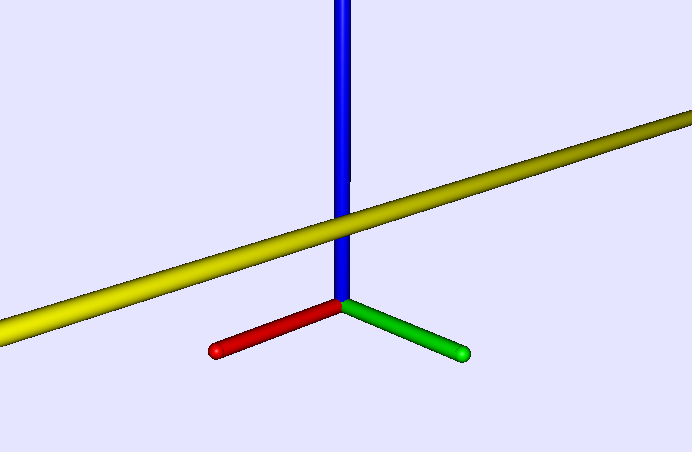
\includegraphics[bb=0 0 346 226 , width=5cm]{Cfig/draw3d.png} 

\hypertarget{connect3d}{}
\vspace{\baselineskip}
\noindent
{\bf 点を結ぶ}:\verb|connect3d(<list>)|

\verb|<list>|で与えられた各点を線分で結ぶ。

\vspace{\baselineskip}
 %%% /Users/hannya/Desktop/fig/s0301table.tex 
%%% Generator=s0301table.cdy 
{\unitlength=1cm%
\begin{picture}%
(12,3)(0,0)%
\special{pn 8}%
%
\special{pa     0 -1181}\special{pa     0    -0}%
\special{fp}%
\special{pa   787 -1181}\special{pa   787    -0}%
\special{fp}%
\special{pa  2756 -1181}\special{pa  2756    -0}%
\special{fp}%
\special{pa  4724 -1181}\special{pa  4724    -0}%
\special{fp}%
\special{pa     0 -1181}\special{pa  4724 -1181}%
\special{fp}%
\special{pa     0  -886}\special{pa  4724  -886}%
\special{fp}%
\special{pa     0  -591}\special{pa  4724  -591}%
\special{fp}%
\special{pa     0  -295}\special{pa  4724  -295}%
\special{fp}%
\special{pa     0    -0}\special{pa  4724    -0}%
\special{fp}%
\settowidth{\Width}{修飾子}\setlength{\Width}{-0.5\Width}%
\settoheight{\Height}{修飾子}\settodepth{\Depth}{修飾子}\setlength{\Height}{-0.5\Height}\setlength{\Depth}{0.5\Depth}\addtolength{\Height}{\Depth}%
\put(  1.000,  2.620){\hspace*{\Width}\raisebox{\Height}{修飾子}}%
%
\settowidth{\Width}{値}\setlength{\Width}{-0.5\Width}%
\settoheight{\Height}{値}\settodepth{\Depth}{値}\setlength{\Height}{-0.5\Height}\setlength{\Depth}{0.5\Depth}\addtolength{\Height}{\Depth}%
\put(  4.500,  2.620){\hspace*{\Width}\raisebox{\Height}{値}}%
%
\settowidth{\Width}{効果}\setlength{\Width}{-0.5\Width}%
\settoheight{\Height}{効果}\settodepth{\Depth}{効果}\setlength{\Height}{-0.5\Height}\setlength{\Depth}{0.5\Depth}\addtolength{\Height}{\Depth}%
\put(  9.500,  2.620){\hspace*{\Width}\raisebox{\Height}{効果}}%
%
\settowidth{\Width}{size}\setlength{\Width}{-0.5\Width}%
\settoheight{\Height}{size}\settodepth{\Depth}{size}\setlength{\Height}{-0.5\Height}\setlength{\Depth}{0.5\Depth}\addtolength{\Height}{\Depth}%
\put(  1.000,  1.880){\hspace*{\Width}\raisebox{\Height}{size}}%
%
\settowidth{\Width}{<real>}\setlength{\Width}{-0.5\Width}%
\settoheight{\Height}{<real>}\settodepth{\Depth}{<real>}\setlength{\Height}{-0.5\Height}\setlength{\Depth}{0.5\Depth}\addtolength{\Height}{\Depth}%
\put(  4.500,  1.880){\hspace*{\Width}\raisebox{\Height}{<real>}}%
%
\settowidth{\Width}{ 線の太さを指定する}\setlength{\Width}{0\Width}%
\settoheight{\Height}{ 線の太さを指定する}\settodepth{\Depth}{ 線の太さを指定する}\setlength{\Height}{-0.5\Height}\setlength{\Depth}{0.5\Depth}\addtolength{\Height}{\Depth}%
\put(  7.050,  1.880){\hspace*{\Width}\raisebox{\Height}{ 線の太さを指定する}}%
%
\settowidth{\Width}{color}\setlength{\Width}{-0.5\Width}%
\settoheight{\Height}{color}\settodepth{\Depth}{color}\setlength{\Height}{-0.5\Height}\setlength{\Depth}{0.5\Depth}\addtolength{\Height}{\Depth}%
\put(  1.000,  1.120){\hspace*{\Width}\raisebox{\Height}{color}}%
%
\settowidth{\Width}{[<real>,<real>,<real>]}\setlength{\Width}{-0.5\Width}%
\settoheight{\Height}{[<real>,<real>,<real>]}\settodepth{\Depth}{[<real>,<real>,<real>]}\setlength{\Height}{-0.5\Height}\setlength{\Depth}{0.5\Depth}\addtolength{\Height}{\Depth}%
\put(  4.500,  1.120){\hspace*{\Width}\raisebox{\Height}{[<real>,<real>,<real>]}}%
%
\settowidth{\Width}{ 色をRGBで指定する}\setlength{\Width}{0\Width}%
\settoheight{\Height}{ 色をRGBで指定する}\settodepth{\Depth}{ 色をRGBで指定する}\setlength{\Height}{-0.5\Height}\setlength{\Depth}{0.5\Depth}\addtolength{\Height}{\Depth}%
\put(  7.050,  1.120){\hspace*{\Width}\raisebox{\Height}{ 色をRGBで指定する}}%
%
\settowidth{\Width}{shininess}\setlength{\Width}{-0.5\Width}%
\settoheight{\Height}{shininess}\settodepth{\Depth}{shininess}\setlength{\Height}{-0.5\Height}\setlength{\Depth}{0.5\Depth}\addtolength{\Height}{\Depth}%
\put(  1.000,  0.380){\hspace*{\Width}\raisebox{\Height}{shininess}}%
%
\settowidth{\Width}{<real>}\setlength{\Width}{-0.5\Width}%
\settoheight{\Height}{<real>}\settodepth{\Depth}{<real>}\setlength{\Height}{-0.5\Height}\setlength{\Depth}{0.5\Depth}\addtolength{\Height}{\Depth}%
\put(  4.500,  0.380){\hspace*{\Width}\raisebox{\Height}{<real>}}%
%
\settowidth{\Width}{ 光沢を指定する}\setlength{\Width}{0\Width}%
\settoheight{\Height}{ 光沢を指定する}\settodepth{\Depth}{ 光沢を指定する}\setlength{\Height}{-0.5\Height}\setlength{\Depth}{0.5\Depth}\addtolength{\Height}{\Depth}%
\put(  7.050,  0.380){\hspace*{\Width}\raisebox{\Height}{ 光沢を指定する}}%
%
\end{picture}}%

\hypertarget{drawpoly3d}{}
\vspace{\baselineskip}
\noindent
{\bf 多角形を描く}:\verb|drawpoly3d(<list>)|

\verb|<list>|で与えられた各点を線分で結んで多角形を描く。

\vspace{\baselineskip}
 %%% /Users/hannya/Desktop/fig/s0301table.tex 
%%% Generator=s0301table.cdy 
{\unitlength=1cm%
\begin{picture}%
(12,3)(0,0)%
\special{pn 8}%
%
\special{pa     0 -1181}\special{pa     0    -0}%
\special{fp}%
\special{pa   787 -1181}\special{pa   787    -0}%
\special{fp}%
\special{pa  2756 -1181}\special{pa  2756    -0}%
\special{fp}%
\special{pa  4724 -1181}\special{pa  4724    -0}%
\special{fp}%
\special{pa     0 -1181}\special{pa  4724 -1181}%
\special{fp}%
\special{pa     0  -886}\special{pa  4724  -886}%
\special{fp}%
\special{pa     0  -591}\special{pa  4724  -591}%
\special{fp}%
\special{pa     0  -295}\special{pa  4724  -295}%
\special{fp}%
\special{pa     0    -0}\special{pa  4724    -0}%
\special{fp}%
\settowidth{\Width}{修飾子}\setlength{\Width}{-0.5\Width}%
\settoheight{\Height}{修飾子}\settodepth{\Depth}{修飾子}\setlength{\Height}{-0.5\Height}\setlength{\Depth}{0.5\Depth}\addtolength{\Height}{\Depth}%
\put(  1.000,  2.620){\hspace*{\Width}\raisebox{\Height}{修飾子}}%
%
\settowidth{\Width}{値}\setlength{\Width}{-0.5\Width}%
\settoheight{\Height}{値}\settodepth{\Depth}{値}\setlength{\Height}{-0.5\Height}\setlength{\Depth}{0.5\Depth}\addtolength{\Height}{\Depth}%
\put(  4.500,  2.620){\hspace*{\Width}\raisebox{\Height}{値}}%
%
\settowidth{\Width}{効果}\setlength{\Width}{-0.5\Width}%
\settoheight{\Height}{効果}\settodepth{\Depth}{効果}\setlength{\Height}{-0.5\Height}\setlength{\Depth}{0.5\Depth}\addtolength{\Height}{\Depth}%
\put(  9.500,  2.620){\hspace*{\Width}\raisebox{\Height}{効果}}%
%
\settowidth{\Width}{size}\setlength{\Width}{-0.5\Width}%
\settoheight{\Height}{size}\settodepth{\Depth}{size}\setlength{\Height}{-0.5\Height}\setlength{\Depth}{0.5\Depth}\addtolength{\Height}{\Depth}%
\put(  1.000,  1.880){\hspace*{\Width}\raisebox{\Height}{size}}%
%
\settowidth{\Width}{<real>}\setlength{\Width}{-0.5\Width}%
\settoheight{\Height}{<real>}\settodepth{\Depth}{<real>}\setlength{\Height}{-0.5\Height}\setlength{\Depth}{0.5\Depth}\addtolength{\Height}{\Depth}%
\put(  4.500,  1.880){\hspace*{\Width}\raisebox{\Height}{<real>}}%
%
\settowidth{\Width}{ 線の太さを指定する}\setlength{\Width}{0\Width}%
\settoheight{\Height}{ 線の太さを指定する}\settodepth{\Depth}{ 線の太さを指定する}\setlength{\Height}{-0.5\Height}\setlength{\Depth}{0.5\Depth}\addtolength{\Height}{\Depth}%
\put(  7.050,  1.880){\hspace*{\Width}\raisebox{\Height}{ 線の太さを指定する}}%
%
\settowidth{\Width}{color}\setlength{\Width}{-0.5\Width}%
\settoheight{\Height}{color}\settodepth{\Depth}{color}\setlength{\Height}{-0.5\Height}\setlength{\Depth}{0.5\Depth}\addtolength{\Height}{\Depth}%
\put(  1.000,  1.120){\hspace*{\Width}\raisebox{\Height}{color}}%
%
\settowidth{\Width}{[<real>,<real>,<real>]}\setlength{\Width}{-0.5\Width}%
\settoheight{\Height}{[<real>,<real>,<real>]}\settodepth{\Depth}{[<real>,<real>,<real>]}\setlength{\Height}{-0.5\Height}\setlength{\Depth}{0.5\Depth}\addtolength{\Height}{\Depth}%
\put(  4.500,  1.120){\hspace*{\Width}\raisebox{\Height}{[<real>,<real>,<real>]}}%
%
\settowidth{\Width}{ 色をRGBで指定する}\setlength{\Width}{0\Width}%
\settoheight{\Height}{ 色をRGBで指定する}\settodepth{\Depth}{ 色をRGBで指定する}\setlength{\Height}{-0.5\Height}\setlength{\Depth}{0.5\Depth}\addtolength{\Height}{\Depth}%
\put(  7.050,  1.120){\hspace*{\Width}\raisebox{\Height}{ 色をRGBで指定する}}%
%
\settowidth{\Width}{shininess}\setlength{\Width}{-0.5\Width}%
\settoheight{\Height}{shininess}\settodepth{\Depth}{shininess}\setlength{\Height}{-0.5\Height}\setlength{\Depth}{0.5\Depth}\addtolength{\Height}{\Depth}%
\put(  1.000,  0.380){\hspace*{\Width}\raisebox{\Height}{shininess}}%
%
\settowidth{\Width}{<real>}\setlength{\Width}{-0.5\Width}%
\settoheight{\Height}{<real>}\settodepth{\Depth}{<real>}\setlength{\Height}{-0.5\Height}\setlength{\Depth}{0.5\Depth}\addtolength{\Height}{\Depth}%
\put(  4.500,  0.380){\hspace*{\Width}\raisebox{\Height}{<real>}}%
%
\settowidth{\Width}{ 光沢を指定する}\setlength{\Width}{0\Width}%
\settoheight{\Height}{ 光沢を指定する}\settodepth{\Depth}{ 光沢を指定する}\setlength{\Height}{-0.5\Height}\setlength{\Depth}{0.5\Depth}\addtolength{\Height}{\Depth}%
\put(  7.050,  0.380){\hspace*{\Width}\raisebox{\Height}{ 光沢を指定する}}%
%
\end{picture}}%

\hypertarget{fillpoly3d}{}
\vspace{\baselineskip}
\noindent
{\bf 多角形の面を描く}:\verb|fillpoly3d(<list>)|

\verb|<list>|で与えられた各点を線分で結んで多角形の面を描く。

\vspace{\baselineskip}
 %%% /Users/hannya/Desktop/fig/s0301table.tex 
%%% Generator=s0301table.cdy 
{\unitlength=1cm%
\begin{picture}%
(12,4)(0,0)%
\special{pn 8}%
%
\special{pa     0 -1575}\special{pa     0    -0}%
\special{fp}%
\special{pa   787 -1575}\special{pa   787    -0}%
\special{fp}%
\special{pa  2756 -1575}\special{pa  2756    -0}%
\special{fp}%
\special{pa  4724 -1575}\special{pa  4724    -0}%
\special{fp}%
\special{pa     0 -1575}\special{pa  4724 -1575}%
\special{fp}%
\special{pa     0 -1260}\special{pa  4724 -1260}%
\special{fp}%
\special{pa     0  -945}\special{pa  4724  -945}%
\special{fp}%
\special{pa     0  -630}\special{pa  4724  -630}%
\special{fp}%
\special{pa     0  -315}\special{pa  4724  -315}%
\special{fp}%
\special{pa     0    -0}\special{pa  4724    -0}%
\special{fp}%
\settowidth{\Width}{修飾子}\setlength{\Width}{-0.5\Width}%
\settoheight{\Height}{修飾子}\settodepth{\Depth}{修飾子}\setlength{\Height}{-0.5\Height}\setlength{\Depth}{0.5\Depth}\addtolength{\Height}{\Depth}%
\put(  1.000,  3.600){\hspace*{\Width}\raisebox{\Height}{修飾子}}%
%
\settowidth{\Width}{値}\setlength{\Width}{-0.5\Width}%
\settoheight{\Height}{値}\settodepth{\Depth}{値}\setlength{\Height}{-0.5\Height}\setlength{\Depth}{0.5\Depth}\addtolength{\Height}{\Depth}%
\put(  4.500,  3.600){\hspace*{\Width}\raisebox{\Height}{値}}%
%
\settowidth{\Width}{効果}\setlength{\Width}{-0.5\Width}%
\settoheight{\Height}{効果}\settodepth{\Depth}{効果}\setlength{\Height}{-0.5\Height}\setlength{\Depth}{0.5\Depth}\addtolength{\Height}{\Depth}%
\put(  9.500,  3.600){\hspace*{\Width}\raisebox{\Height}{効果}}%
%
\settowidth{\Width}{size}\setlength{\Width}{-0.5\Width}%
\settoheight{\Height}{size}\settodepth{\Depth}{size}\setlength{\Height}{-0.5\Height}\setlength{\Depth}{0.5\Depth}\addtolength{\Height}{\Depth}%
\put(  1.000,  2.800){\hspace*{\Width}\raisebox{\Height}{size}}%
%
\settowidth{\Width}{<real>}\setlength{\Width}{-0.5\Width}%
\settoheight{\Height}{<real>}\settodepth{\Depth}{<real>}\setlength{\Height}{-0.5\Height}\setlength{\Depth}{0.5\Depth}\addtolength{\Height}{\Depth}%
\put(  4.500,  2.800){\hspace*{\Width}\raisebox{\Height}{<real>}}%
%
\settowidth{\Width}{ 面の大きさを指定する}\setlength{\Width}{0\Width}%
\settoheight{\Height}{ 面の大きさを指定する}\settodepth{\Depth}{ 面の大きさを指定する}\setlength{\Height}{-0.5\Height}\setlength{\Depth}{0.5\Depth}\addtolength{\Height}{\Depth}%
\put(  7.050,  2.800){\hspace*{\Width}\raisebox{\Height}{ 面の大きさを指定する}}%
%
\settowidth{\Width}{color}\setlength{\Width}{-0.5\Width}%
\settoheight{\Height}{color}\settodepth{\Depth}{color}\setlength{\Height}{-0.5\Height}\setlength{\Depth}{0.5\Depth}\addtolength{\Height}{\Depth}%
\put(  1.000,  2.000){\hspace*{\Width}\raisebox{\Height}{color}}%
%
\settowidth{\Width}{[<real>,<real>,<real>]}\setlength{\Width}{-0.5\Width}%
\settoheight{\Height}{[<real>,<real>,<real>]}\settodepth{\Depth}{[<real>,<real>,<real>]}\setlength{\Height}{-0.5\Height}\setlength{\Depth}{0.5\Depth}\addtolength{\Height}{\Depth}%
\put(  4.500,  2.000){\hspace*{\Width}\raisebox{\Height}{[<real>,<real>,<real>]}}%
%
\settowidth{\Width}{ 色をRGBで指定する}\setlength{\Width}{0\Width}%
\settoheight{\Height}{ 色をRGBで指定する}\settodepth{\Depth}{ 色をRGBで指定する}\setlength{\Height}{-0.5\Height}\setlength{\Depth}{0.5\Depth}\addtolength{\Height}{\Depth}%
\put(  7.050,  2.000){\hspace*{\Width}\raisebox{\Height}{ 色をRGBで指定する}}%
%
\settowidth{\Width}{shininess}\setlength{\Width}{-0.5\Width}%
\settoheight{\Height}{shininess}\settodepth{\Depth}{shininess}\setlength{\Height}{-0.5\Height}\setlength{\Depth}{0.5\Depth}\addtolength{\Height}{\Depth}%
\put(  1.000,  1.200){\hspace*{\Width}\raisebox{\Height}{shininess}}%
%
\settowidth{\Width}{<real>}\setlength{\Width}{-0.5\Width}%
\settoheight{\Height}{<real>}\settodepth{\Depth}{<real>}\setlength{\Height}{-0.5\Height}\setlength{\Depth}{0.5\Depth}\addtolength{\Height}{\Depth}%
\put(  4.500,  1.200){\hspace*{\Width}\raisebox{\Height}{<real>}}%
%
\settowidth{\Width}{ 光沢を指定する}\setlength{\Width}{0\Width}%
\settoheight{\Height}{ 光沢を指定する}\settodepth{\Depth}{ 光沢を指定する}\setlength{\Height}{-0.5\Height}\setlength{\Depth}{0.5\Depth}\addtolength{\Height}{\Depth}%
\put(  7.050,  1.200){\hspace*{\Width}\raisebox{\Height}{ 光沢を指定する}}%
%
\settowidth{\Width}{alpha}\setlength{\Width}{-0.5\Width}%
\settoheight{\Height}{alpha}\settodepth{\Depth}{alpha}\setlength{\Height}{-0.5\Height}\setlength{\Depth}{0.5\Depth}\addtolength{\Height}{\Depth}%
\put(  1.000,  0.400){\hspace*{\Width}\raisebox{\Height}{alpha}}%
%
\settowidth{\Width}{<real>}\setlength{\Width}{-0.5\Width}%
\settoheight{\Height}{<real>}\settodepth{\Depth}{<real>}\setlength{\Height}{-0.5\Height}\setlength{\Depth}{0.5\Depth}\addtolength{\Height}{\Depth}%
\put(  4.500,  0.400){\hspace*{\Width}\raisebox{\Height}{<real>}}%
%
\settowidth{\Width}{ 透明度を指定する}\setlength{\Width}{0\Width}%
\settoheight{\Height}{ 透明度を指定する}\settodepth{\Depth}{ 透明度を指定する}\setlength{\Height}{-0.5\Height}\setlength{\Depth}{0.5\Depth}\addtolength{\Height}{\Depth}%
\put(  7.050,  0.400){\hspace*{\Width}\raisebox{\Height}{ 透明度を指定する}}%
%
\end{picture}}%

\vspace{\baselineskip}
\noindent
{\bf 法線ベクトルを指定して多角形の面を描く}:\verb|fillpoly3d(<list1>,<list2>)|

ユーザー定義の法線ベクトルによる多角形の面を描く。法線ベクトルは、光の当たり方を計算するものである。

\verb|<list1>|は多角形の頂点の座標,\verb|<list2>| は多角形の各頂点の法線ベクトル。 \verb|<list1>| と \verb|<list2>| の長さは一致する必要がある。

\vspace{\baselineskip}
 %%% /Users/hannya/Desktop/fig/s0301table.tex 
%%% Generator=s0301table.cdy 
{\unitlength=1cm%
\begin{picture}%
(12,4)(0,0)%
\special{pn 8}%
%
\special{pa     0 -1575}\special{pa     0    -0}%
\special{fp}%
\special{pa   787 -1575}\special{pa   787    -0}%
\special{fp}%
\special{pa  2756 -1575}\special{pa  2756    -0}%
\special{fp}%
\special{pa  4724 -1575}\special{pa  4724    -0}%
\special{fp}%
\special{pa     0 -1575}\special{pa  4724 -1575}%
\special{fp}%
\special{pa     0 -1260}\special{pa  4724 -1260}%
\special{fp}%
\special{pa     0  -945}\special{pa  4724  -945}%
\special{fp}%
\special{pa     0  -630}\special{pa  4724  -630}%
\special{fp}%
\special{pa     0  -315}\special{pa  4724  -315}%
\special{fp}%
\special{pa     0    -0}\special{pa  4724    -0}%
\special{fp}%
\settowidth{\Width}{修飾子}\setlength{\Width}{-0.5\Width}%
\settoheight{\Height}{修飾子}\settodepth{\Depth}{修飾子}\setlength{\Height}{-0.5\Height}\setlength{\Depth}{0.5\Depth}\addtolength{\Height}{\Depth}%
\put(  1.000,  3.600){\hspace*{\Width}\raisebox{\Height}{修飾子}}%
%
\settowidth{\Width}{値}\setlength{\Width}{-0.5\Width}%
\settoheight{\Height}{値}\settodepth{\Depth}{値}\setlength{\Height}{-0.5\Height}\setlength{\Depth}{0.5\Depth}\addtolength{\Height}{\Depth}%
\put(  4.500,  3.600){\hspace*{\Width}\raisebox{\Height}{値}}%
%
\settowidth{\Width}{効果}\setlength{\Width}{-0.5\Width}%
\settoheight{\Height}{効果}\settodepth{\Depth}{効果}\setlength{\Height}{-0.5\Height}\setlength{\Depth}{0.5\Depth}\addtolength{\Height}{\Depth}%
\put(  9.500,  3.600){\hspace*{\Width}\raisebox{\Height}{効果}}%
%
\settowidth{\Width}{size}\setlength{\Width}{-0.5\Width}%
\settoheight{\Height}{size}\settodepth{\Depth}{size}\setlength{\Height}{-0.5\Height}\setlength{\Depth}{0.5\Depth}\addtolength{\Height}{\Depth}%
\put(  1.000,  2.800){\hspace*{\Width}\raisebox{\Height}{size}}%
%
\settowidth{\Width}{<real>}\setlength{\Width}{-0.5\Width}%
\settoheight{\Height}{<real>}\settodepth{\Depth}{<real>}\setlength{\Height}{-0.5\Height}\setlength{\Depth}{0.5\Depth}\addtolength{\Height}{\Depth}%
\put(  4.500,  2.800){\hspace*{\Width}\raisebox{\Height}{<real>}}%
%
\settowidth{\Width}{ 面の大きさを指定する}\setlength{\Width}{0\Width}%
\settoheight{\Height}{ 面の大きさを指定する}\settodepth{\Depth}{ 面の大きさを指定する}\setlength{\Height}{-0.5\Height}\setlength{\Depth}{0.5\Depth}\addtolength{\Height}{\Depth}%
\put(  7.050,  2.800){\hspace*{\Width}\raisebox{\Height}{ 面の大きさを指定する}}%
%
\settowidth{\Width}{color}\setlength{\Width}{-0.5\Width}%
\settoheight{\Height}{color}\settodepth{\Depth}{color}\setlength{\Height}{-0.5\Height}\setlength{\Depth}{0.5\Depth}\addtolength{\Height}{\Depth}%
\put(  1.000,  2.000){\hspace*{\Width}\raisebox{\Height}{color}}%
%
\settowidth{\Width}{[<real>,<real>,<real>]}\setlength{\Width}{-0.5\Width}%
\settoheight{\Height}{[<real>,<real>,<real>]}\settodepth{\Depth}{[<real>,<real>,<real>]}\setlength{\Height}{-0.5\Height}\setlength{\Depth}{0.5\Depth}\addtolength{\Height}{\Depth}%
\put(  4.500,  2.000){\hspace*{\Width}\raisebox{\Height}{[<real>,<real>,<real>]}}%
%
\settowidth{\Width}{ 色をRGBで指定する}\setlength{\Width}{0\Width}%
\settoheight{\Height}{ 色をRGBで指定する}\settodepth{\Depth}{ 色をRGBで指定する}\setlength{\Height}{-0.5\Height}\setlength{\Depth}{0.5\Depth}\addtolength{\Height}{\Depth}%
\put(  7.050,  2.000){\hspace*{\Width}\raisebox{\Height}{ 色をRGBで指定する}}%
%
\settowidth{\Width}{shininess}\setlength{\Width}{-0.5\Width}%
\settoheight{\Height}{shininess}\settodepth{\Depth}{shininess}\setlength{\Height}{-0.5\Height}\setlength{\Depth}{0.5\Depth}\addtolength{\Height}{\Depth}%
\put(  1.000,  1.200){\hspace*{\Width}\raisebox{\Height}{shininess}}%
%
\settowidth{\Width}{<real>}\setlength{\Width}{-0.5\Width}%
\settoheight{\Height}{<real>}\settodepth{\Depth}{<real>}\setlength{\Height}{-0.5\Height}\setlength{\Depth}{0.5\Depth}\addtolength{\Height}{\Depth}%
\put(  4.500,  1.200){\hspace*{\Width}\raisebox{\Height}{<real>}}%
%
\settowidth{\Width}{ 光沢を指定する}\setlength{\Width}{0\Width}%
\settoheight{\Height}{ 光沢を指定する}\settodepth{\Depth}{ 光沢を指定する}\setlength{\Height}{-0.5\Height}\setlength{\Depth}{0.5\Depth}\addtolength{\Height}{\Depth}%
\put(  7.050,  1.200){\hspace*{\Width}\raisebox{\Height}{ 光沢を指定する}}%
%
\settowidth{\Width}{alpha}\setlength{\Width}{-0.5\Width}%
\settoheight{\Height}{alpha}\settodepth{\Depth}{alpha}\setlength{\Height}{-0.5\Height}\setlength{\Depth}{0.5\Depth}\addtolength{\Height}{\Depth}%
\put(  1.000,  0.400){\hspace*{\Width}\raisebox{\Height}{alpha}}%
%
\settowidth{\Width}{<real>}\setlength{\Width}{-0.5\Width}%
\settoheight{\Height}{<real>}\settodepth{\Depth}{<real>}\setlength{\Height}{-0.5\Height}\setlength{\Depth}{0.5\Depth}\addtolength{\Height}{\Depth}%
\put(  4.500,  0.400){\hspace*{\Width}\raisebox{\Height}{<real>}}%
%
\settowidth{\Width}{ 透明度を指定する}\setlength{\Width}{0\Width}%
\settoheight{\Height}{ 透明度を指定する}\settodepth{\Depth}{ 透明度を指定する}\setlength{\Height}{-0.5\Height}\setlength{\Depth}{0.5\Depth}\addtolength{\Height}{\Depth}%
\put(  7.050,  0.400){\hspace*{\Width}\raisebox{\Height}{ 透明度を指定する}}%
%
\end{picture}}%

\hypertarget{fillcircle3d}{}
\vspace{\baselineskip}
\noindent
{\bf 円盤を描く}:\verb|fillcircle3d(<point>,<vec>,<real>)|

\verb|<point>|を中心、\verb|<vec>|を法線ベクトル、\verb|<real>|を半径とする円盤を描く。

\vspace{\baselineskip}
 %%% /Users/hannya/Desktop/fig/s0301table.tex 
%%% Generator=s0301table.cdy 
{\unitlength=1cm%
\begin{picture}%
(12,4)(0,0)%
\special{pn 8}%
%
\special{pa     0 -1575}\special{pa     0    -0}%
\special{fp}%
\special{pa   787 -1575}\special{pa   787    -0}%
\special{fp}%
\special{pa  2756 -1575}\special{pa  2756    -0}%
\special{fp}%
\special{pa  4724 -1575}\special{pa  4724    -0}%
\special{fp}%
\special{pa     0 -1575}\special{pa  4724 -1575}%
\special{fp}%
\special{pa     0 -1260}\special{pa  4724 -1260}%
\special{fp}%
\special{pa     0  -945}\special{pa  4724  -945}%
\special{fp}%
\special{pa     0  -630}\special{pa  4724  -630}%
\special{fp}%
\special{pa     0  -315}\special{pa  4724  -315}%
\special{fp}%
\special{pa     0    -0}\special{pa  4724    -0}%
\special{fp}%
\settowidth{\Width}{修飾子}\setlength{\Width}{-0.5\Width}%
\settoheight{\Height}{修飾子}\settodepth{\Depth}{修飾子}\setlength{\Height}{-0.5\Height}\setlength{\Depth}{0.5\Depth}\addtolength{\Height}{\Depth}%
\put(  1.000,  3.600){\hspace*{\Width}\raisebox{\Height}{修飾子}}%
%
\settowidth{\Width}{値}\setlength{\Width}{-0.5\Width}%
\settoheight{\Height}{値}\settodepth{\Depth}{値}\setlength{\Height}{-0.5\Height}\setlength{\Depth}{0.5\Depth}\addtolength{\Height}{\Depth}%
\put(  4.500,  3.600){\hspace*{\Width}\raisebox{\Height}{値}}%
%
\settowidth{\Width}{効果}\setlength{\Width}{-0.5\Width}%
\settoheight{\Height}{効果}\settodepth{\Depth}{効果}\setlength{\Height}{-0.5\Height}\setlength{\Depth}{0.5\Depth}\addtolength{\Height}{\Depth}%
\put(  9.500,  3.600){\hspace*{\Width}\raisebox{\Height}{効果}}%
%
\settowidth{\Width}{size}\setlength{\Width}{-0.5\Width}%
\settoheight{\Height}{size}\settodepth{\Depth}{size}\setlength{\Height}{-0.5\Height}\setlength{\Depth}{0.5\Depth}\addtolength{\Height}{\Depth}%
\put(  1.000,  2.800){\hspace*{\Width}\raisebox{\Height}{size}}%
%
\settowidth{\Width}{<real>}\setlength{\Width}{-0.5\Width}%
\settoheight{\Height}{<real>}\settodepth{\Depth}{<real>}\setlength{\Height}{-0.5\Height}\setlength{\Depth}{0.5\Depth}\addtolength{\Height}{\Depth}%
\put(  4.500,  2.800){\hspace*{\Width}\raisebox{\Height}{<real>}}%
%
\settowidth{\Width}{ 面の大きさを指定する}\setlength{\Width}{0\Width}%
\settoheight{\Height}{ 面の大きさを指定する}\settodepth{\Depth}{ 面の大きさを指定する}\setlength{\Height}{-0.5\Height}\setlength{\Depth}{0.5\Depth}\addtolength{\Height}{\Depth}%
\put(  7.050,  2.800){\hspace*{\Width}\raisebox{\Height}{ 面の大きさを指定する}}%
%
\settowidth{\Width}{color}\setlength{\Width}{-0.5\Width}%
\settoheight{\Height}{color}\settodepth{\Depth}{color}\setlength{\Height}{-0.5\Height}\setlength{\Depth}{0.5\Depth}\addtolength{\Height}{\Depth}%
\put(  1.000,  2.000){\hspace*{\Width}\raisebox{\Height}{color}}%
%
\settowidth{\Width}{[<real>,<real>,<real>]}\setlength{\Width}{-0.5\Width}%
\settoheight{\Height}{[<real>,<real>,<real>]}\settodepth{\Depth}{[<real>,<real>,<real>]}\setlength{\Height}{-0.5\Height}\setlength{\Depth}{0.5\Depth}\addtolength{\Height}{\Depth}%
\put(  4.500,  2.000){\hspace*{\Width}\raisebox{\Height}{[<real>,<real>,<real>]}}%
%
\settowidth{\Width}{ 色をRGBで指定する}\setlength{\Width}{0\Width}%
\settoheight{\Height}{ 色をRGBで指定する}\settodepth{\Depth}{ 色をRGBで指定する}\setlength{\Height}{-0.5\Height}\setlength{\Depth}{0.5\Depth}\addtolength{\Height}{\Depth}%
\put(  7.050,  2.000){\hspace*{\Width}\raisebox{\Height}{ 色をRGBで指定する}}%
%
\settowidth{\Width}{shininess}\setlength{\Width}{-0.5\Width}%
\settoheight{\Height}{shininess}\settodepth{\Depth}{shininess}\setlength{\Height}{-0.5\Height}\setlength{\Depth}{0.5\Depth}\addtolength{\Height}{\Depth}%
\put(  1.000,  1.200){\hspace*{\Width}\raisebox{\Height}{shininess}}%
%
\settowidth{\Width}{<real>}\setlength{\Width}{-0.5\Width}%
\settoheight{\Height}{<real>}\settodepth{\Depth}{<real>}\setlength{\Height}{-0.5\Height}\setlength{\Depth}{0.5\Depth}\addtolength{\Height}{\Depth}%
\put(  4.500,  1.200){\hspace*{\Width}\raisebox{\Height}{<real>}}%
%
\settowidth{\Width}{ 光沢を指定する}\setlength{\Width}{0\Width}%
\settoheight{\Height}{ 光沢を指定する}\settodepth{\Depth}{ 光沢を指定する}\setlength{\Height}{-0.5\Height}\setlength{\Depth}{0.5\Depth}\addtolength{\Height}{\Depth}%
\put(  7.050,  1.200){\hspace*{\Width}\raisebox{\Height}{ 光沢を指定する}}%
%
\settowidth{\Width}{alpha}\setlength{\Width}{-0.5\Width}%
\settoheight{\Height}{alpha}\settodepth{\Depth}{alpha}\setlength{\Height}{-0.5\Height}\setlength{\Depth}{0.5\Depth}\addtolength{\Height}{\Depth}%
\put(  1.000,  0.400){\hspace*{\Width}\raisebox{\Height}{alpha}}%
%
\settowidth{\Width}{<real>}\setlength{\Width}{-0.5\Width}%
\settoheight{\Height}{<real>}\settodepth{\Depth}{<real>}\setlength{\Height}{-0.5\Height}\setlength{\Depth}{0.5\Depth}\addtolength{\Height}{\Depth}%
\put(  4.500,  0.400){\hspace*{\Width}\raisebox{\Height}{<real>}}%
%
\settowidth{\Width}{ 透明度を指定する}\setlength{\Width}{0\Width}%
\settoheight{\Height}{ 透明度を指定する}\settodepth{\Depth}{ 透明度を指定する}\setlength{\Height}{-0.5\Height}\setlength{\Depth}{0.5\Depth}\addtolength{\Height}{\Depth}%
\put(  7.050,  0.400){\hspace*{\Width}\raisebox{\Height}{ 透明度を指定する}}%
%
\end{picture}}%

\vspace{\baselineskip}
\noindent
【例】座標軸と円盤を描く。

Initialization スロットに次のコードを書く。以後の例も同様。

\begin{verbatim}
  use("Cindy3D");
  background3d([0.9,0.9,1]);
  renderhints3d(quality->4);
  lookat3d([4,4,4],[0,0,0],[-1,-1,0]);
\end{verbatim}

drawスロットに次のコードを書く。

\begin{verbatim}
  renderhints3d(quality->4);
  begin3d();
  draw3d([0,0,0],[3,0,0],color->[1,0,0],size->0.3);  // 座標軸
  draw3d([0,0,0],[0,3,0],color->[0,1,0],size->0.3);
  draw3d([0,0,0],[0,0,3],color->[0,0,1],size->0.3);
  fillcircle3d([sqrt(3)/6,sqrt(3)/6,sqrt(3)/6],[1,1,1],
    sqrt(3)/2,color->[1,0,0],alpha->0.3);
  end3d()
\end{verbatim}

\verb|renderhints3d(quality->4)| はレンダリングの品質を指定する関数。(後述)

左が実行結果。右はマウスで画面上をドラッグし,回転したもの。

\vspace{\baselineskip}
\hspace{10mm} 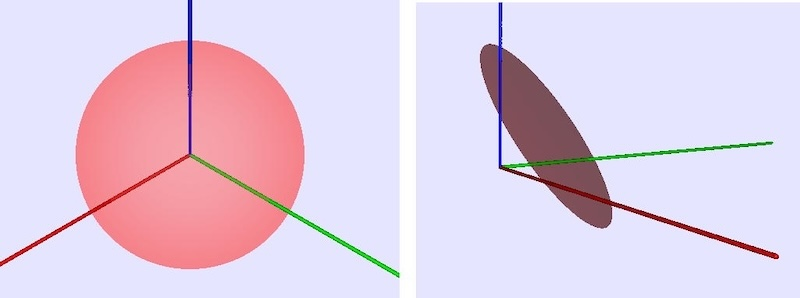
\includegraphics[bb=0 0 800 298 , width=10cm]{Cfig/fillcircle.jpg} 

\hypertarget{drawsphere3d}{}
\vspace{\baselineskip}
\noindent
{\bf 球面を描く}:\verb|drawsphere3d(<point>,<real>)|

\verb|<point>|を中心、\verb|<real>|を半径とする球面を描く。

\vspace{\baselineskip}
 %%% /Users/hannya/Desktop/fig/s0301table.tex 
%%% Generator=s0301table.cdy 
{\unitlength=1cm%
\begin{picture}%
(12,4)(0,0)%
\special{pn 8}%
%
\special{pa     0 -1575}\special{pa     0    -0}%
\special{fp}%
\special{pa   787 -1575}\special{pa   787    -0}%
\special{fp}%
\special{pa  2756 -1575}\special{pa  2756    -0}%
\special{fp}%
\special{pa  4724 -1575}\special{pa  4724    -0}%
\special{fp}%
\special{pa     0 -1575}\special{pa  4724 -1575}%
\special{fp}%
\special{pa     0 -1260}\special{pa  4724 -1260}%
\special{fp}%
\special{pa     0  -945}\special{pa  4724  -945}%
\special{fp}%
\special{pa     0  -630}\special{pa  4724  -630}%
\special{fp}%
\special{pa     0  -315}\special{pa  4724  -315}%
\special{fp}%
\special{pa     0    -0}\special{pa  4724    -0}%
\special{fp}%
\settowidth{\Width}{修飾子}\setlength{\Width}{-0.5\Width}%
\settoheight{\Height}{修飾子}\settodepth{\Depth}{修飾子}\setlength{\Height}{-0.5\Height}\setlength{\Depth}{0.5\Depth}\addtolength{\Height}{\Depth}%
\put(  1.000,  3.600){\hspace*{\Width}\raisebox{\Height}{修飾子}}%
%
\settowidth{\Width}{値}\setlength{\Width}{-0.5\Width}%
\settoheight{\Height}{値}\settodepth{\Depth}{値}\setlength{\Height}{-0.5\Height}\setlength{\Depth}{0.5\Depth}\addtolength{\Height}{\Depth}%
\put(  4.500,  3.600){\hspace*{\Width}\raisebox{\Height}{値}}%
%
\settowidth{\Width}{効果}\setlength{\Width}{-0.5\Width}%
\settoheight{\Height}{効果}\settodepth{\Depth}{効果}\setlength{\Height}{-0.5\Height}\setlength{\Depth}{0.5\Depth}\addtolength{\Height}{\Depth}%
\put(  9.500,  3.600){\hspace*{\Width}\raisebox{\Height}{効果}}%
%
\settowidth{\Width}{size}\setlength{\Width}{-0.5\Width}%
\settoheight{\Height}{size}\settodepth{\Depth}{size}\setlength{\Height}{-0.5\Height}\setlength{\Depth}{0.5\Depth}\addtolength{\Height}{\Depth}%
\put(  1.000,  2.800){\hspace*{\Width}\raisebox{\Height}{size}}%
%
\settowidth{\Width}{<real>}\setlength{\Width}{-0.5\Width}%
\settoheight{\Height}{<real>}\settodepth{\Depth}{<real>}\setlength{\Height}{-0.5\Height}\setlength{\Depth}{0.5\Depth}\addtolength{\Height}{\Depth}%
\put(  4.500,  2.800){\hspace*{\Width}\raisebox{\Height}{<real>}}%
%
\settowidth{\Width}{ 面の大きさを指定する}\setlength{\Width}{0\Width}%
\settoheight{\Height}{ 面の大きさを指定する}\settodepth{\Depth}{ 面の大きさを指定する}\setlength{\Height}{-0.5\Height}\setlength{\Depth}{0.5\Depth}\addtolength{\Height}{\Depth}%
\put(  7.050,  2.800){\hspace*{\Width}\raisebox{\Height}{ 面の大きさを指定する}}%
%
\settowidth{\Width}{color}\setlength{\Width}{-0.5\Width}%
\settoheight{\Height}{color}\settodepth{\Depth}{color}\setlength{\Height}{-0.5\Height}\setlength{\Depth}{0.5\Depth}\addtolength{\Height}{\Depth}%
\put(  1.000,  2.000){\hspace*{\Width}\raisebox{\Height}{color}}%
%
\settowidth{\Width}{[<real>,<real>,<real>]}\setlength{\Width}{-0.5\Width}%
\settoheight{\Height}{[<real>,<real>,<real>]}\settodepth{\Depth}{[<real>,<real>,<real>]}\setlength{\Height}{-0.5\Height}\setlength{\Depth}{0.5\Depth}\addtolength{\Height}{\Depth}%
\put(  4.500,  2.000){\hspace*{\Width}\raisebox{\Height}{[<real>,<real>,<real>]}}%
%
\settowidth{\Width}{ 色をRGBで指定する}\setlength{\Width}{0\Width}%
\settoheight{\Height}{ 色をRGBで指定する}\settodepth{\Depth}{ 色をRGBで指定する}\setlength{\Height}{-0.5\Height}\setlength{\Depth}{0.5\Depth}\addtolength{\Height}{\Depth}%
\put(  7.050,  2.000){\hspace*{\Width}\raisebox{\Height}{ 色をRGBで指定する}}%
%
\settowidth{\Width}{shininess}\setlength{\Width}{-0.5\Width}%
\settoheight{\Height}{shininess}\settodepth{\Depth}{shininess}\setlength{\Height}{-0.5\Height}\setlength{\Depth}{0.5\Depth}\addtolength{\Height}{\Depth}%
\put(  1.000,  1.200){\hspace*{\Width}\raisebox{\Height}{shininess}}%
%
\settowidth{\Width}{<real>}\setlength{\Width}{-0.5\Width}%
\settoheight{\Height}{<real>}\settodepth{\Depth}{<real>}\setlength{\Height}{-0.5\Height}\setlength{\Depth}{0.5\Depth}\addtolength{\Height}{\Depth}%
\put(  4.500,  1.200){\hspace*{\Width}\raisebox{\Height}{<real>}}%
%
\settowidth{\Width}{ 光沢を指定する}\setlength{\Width}{0\Width}%
\settoheight{\Height}{ 光沢を指定する}\settodepth{\Depth}{ 光沢を指定する}\setlength{\Height}{-0.5\Height}\setlength{\Depth}{0.5\Depth}\addtolength{\Height}{\Depth}%
\put(  7.050,  1.200){\hspace*{\Width}\raisebox{\Height}{ 光沢を指定する}}%
%
\settowidth{\Width}{alpha}\setlength{\Width}{-0.5\Width}%
\settoheight{\Height}{alpha}\settodepth{\Depth}{alpha}\setlength{\Height}{-0.5\Height}\setlength{\Depth}{0.5\Depth}\addtolength{\Height}{\Depth}%
\put(  1.000,  0.400){\hspace*{\Width}\raisebox{\Height}{alpha}}%
%
\settowidth{\Width}{<real>}\setlength{\Width}{-0.5\Width}%
\settoheight{\Height}{<real>}\settodepth{\Depth}{<real>}\setlength{\Height}{-0.5\Height}\setlength{\Depth}{0.5\Depth}\addtolength{\Height}{\Depth}%
\put(  4.500,  0.400){\hspace*{\Width}\raisebox{\Height}{<real>}}%
%
\settowidth{\Width}{ 透明度を指定する}\setlength{\Width}{0\Width}%
\settoheight{\Height}{ 透明度を指定する}\settodepth{\Depth}{ 透明度を指定する}\setlength{\Height}{-0.5\Height}\setlength{\Depth}{0.5\Depth}\addtolength{\Height}{\Depth}%
\put(  7.050,  0.400){\hspace*{\Width}\raisebox{\Height}{ 透明度を指定する}}%
%
\end{picture}}%

\hypertarget{mesh3d}{} 
\vspace{\baselineskip}
\noindent
{\bf 網目上の曲面を描く}:\verb|mesh3d(<int1>,<int2>,<list>)|

曲面を、m行n列の格子点でできる網目状に区切る。(メッシュモデル)

\verb|<int1>| 格子点の行数 m

\verb|<int2>| 格子点の列数 n

\verb|<list>| 格子点のリスト

リストは2次元の格子点のリストを平坦化したもので,リストの長さは m × n 。

\vspace{\baselineskip}
\noindent
【例】図は、5行7列の格子点からなる放物線状の面。修飾子の効果を比較するため、かなり荒い網目にしてある。

\begin{verbatim}
  begin3d();
  pt=apply(-2..2,s,
        apply(-3..3,t,
          y = s/3; 
          x = t/3;
          z = x^2+y^2;
          (x,y,z);
        );
     );
  pt=flatten(pt,levels->1);
  mesh3d(5,7,pt);
  end3d()
\end{verbatim}

\begin{layer}{150}{0}
\putnotese{70}{-60}{
\includegraphics[bb=0 0 321 165 , width=5cm]{Cfig/mesh1.png}}
\end{layer}

\verb|apply|関数のネストにより作成した格子点のリストを、\verb|flattenn()|により平坦化して引数に与えている。

\vspace{\baselineskip}
 %%% /Users/hannya/Desktop/fig/s0301tab.tex 
%%% Generator=s0301tab.cdy 
{\unitlength=1cm%
\begin{picture}%
(12.8,7.6)(0,0)%
\special{pn 8}%
%
\special{pa     0 -2992}\special{pa     0    -0}%
\special{fp}%
\special{pa   709 -2992}\special{pa   709    -0}%
\special{fp}%
\special{pa  2677 -2992}\special{pa  2677    -0}%
\special{fp}%
\special{pa  5039 -2992}\special{pa  5039    -0}%
\special{fp}%
\special{pa     0 -2992}\special{pa  5039 -2992}%
\special{fp}%
\special{pa     0 -2677}\special{pa  5039 -2677}%
\special{fp}%
\special{pa     0 -2047}\special{pa  5039 -2047}%
\special{fp}%
\special{pa     0 -1260}\special{pa  5039 -1260}%
\special{fp}%
\special{pa     0  -945}\special{pa  5039  -945}%
\special{fp}%
\special{pa     0  -630}\special{pa  5039  -630}%
\special{fp}%
\special{pa     0  -315}\special{pa  5039  -315}%
\special{fp}%
\special{pa     0    -0}\special{pa  5039    -0}%
\special{fp}%
\settowidth{\Width}{修飾子}\setlength{\Width}{-0.5\Width}%
\settoheight{\Height}{修飾子}\settodepth{\Depth}{修飾子}\setlength{\Height}{-0.5\Height}\setlength{\Depth}{0.5\Depth}\addtolength{\Height}{\Depth}%
\put(  0.900,  7.200){\hspace*{\Width}\raisebox{\Height}{修飾子}}%
%
\settowidth{\Width}{値}\setlength{\Width}{-0.5\Width}%
\settoheight{\Height}{値}\settodepth{\Depth}{値}\setlength{\Height}{-0.5\Height}\setlength{\Depth}{0.5\Depth}\addtolength{\Height}{\Depth}%
\put(  4.300,  7.200){\hspace*{\Width}\raisebox{\Height}{値}}%
%
\settowidth{\Width}{効果}\setlength{\Width}{-0.5\Width}%
\settoheight{\Height}{効果}\settodepth{\Depth}{効果}\setlength{\Height}{-0.5\Height}\setlength{\Depth}{0.5\Depth}\addtolength{\Height}{\Depth}%
\put(  9.800,  7.200){\hspace*{\Width}\raisebox{\Height}{効果}}%
%
\settowidth{\Width}{nomaltype}\setlength{\Width}{-0.5\Width}%
\settoheight{\Height}{nomaltype}\settodepth{\Depth}{nomaltype}\setlength{\Height}{-0.5\Height}\setlength{\Depth}{0.5\Depth}\addtolength{\Height}{\Depth}%
\put(  0.900,  6.000){\hspace*{\Width}\raisebox{\Height}{nomaltype}}%
%
\settowidth{\Width}{<string>}\setlength{\Width}{-0.5\Width}%
\settoheight{\Height}{<string>}\settodepth{\Depth}{<string>}\setlength{\Height}{-0.5\Height}\setlength{\Depth}{0.5\Depth}\addtolength{\Height}{\Depth}%
\put(  4.300,  6.000){\hspace*{\Width}\raisebox{\Height}{<string>}}%
%
\settowidth{\Width}{ \begin{minipage}{60mm}法線のタイプを指定する。値は\\ "perface" , "pervertex"  \end{minipage}}\setlength{\Width}{0\Width}%
\settoheight{\Height}{ \begin{minipage}{60mm}法線のタイプを指定する。値は\\ "perface" , "pervertex"  \end{minipage}}\settodepth{\Depth}{ \begin{minipage}{60mm}法線のタイプを指定する。値は\\ "perface" , "pervertex"  \end{minipage}}\setlength{\Height}{-0.5\Height}\setlength{\Depth}{0.5\Depth}\addtolength{\Height}{\Depth}%
\put(  6.850,  6.000){\hspace*{\Width}\raisebox{\Height}{ \begin{minipage}{60mm}法線のタイプを指定する。値は\\ "perface" , "pervertex"  \end{minipage}}}%
%
\settowidth{\Width}{topology}\setlength{\Width}{-0.5\Width}%
\settoheight{\Height}{topology}\settodepth{\Depth}{topology}\setlength{\Height}{-0.5\Height}\setlength{\Depth}{0.5\Depth}\addtolength{\Height}{\Depth}%
\put(  0.900,  4.200){\hspace*{\Width}\raisebox{\Height}{topology}}%
%
\settowidth{\Width}{<string>}\setlength{\Width}{-0.5\Width}%
\settoheight{\Height}{<string>}\settodepth{\Depth}{<string>}\setlength{\Height}{-0.5\Height}\setlength{\Depth}{0.5\Depth}\addtolength{\Height}{\Depth}%
\put(  4.300,  4.200){\hspace*{\Width}\raisebox{\Height}{<string>}}%
%
\settowidth{\Width}{ \begin{minipage}{70mm}topologyを指定する。値は\\ "open", "closerows", closerolumns,\\ "closeboth"  のいずれか \end{minipage}}\setlength{\Width}{0\Width}%
\settoheight{\Height}{ \begin{minipage}{70mm}topologyを指定する。値は\\ "open", "closerows", "closecolumns",\\ "closeboth"  のいずれか \end{minipage}}\settodepth{\Depth}{ \begin{minipage}{70mm}topologyを指定する。値は\\ "open", closecows, "closecolumns",\\ "closeboth"  のいずれか \end{minipage}}\setlength{\Height}{-0.5\Height}\setlength{\Depth}{0.5\Depth}\addtolength{\Height}{\Depth}%
\put(  6.850,  4.200){\hspace*{\Width}\raisebox{\Height}{ \begin{minipage}{70mm}topologyを指定する。値は\\ "open", "closerows", "closecolumns",\\ "closeboth"  のいずれか \end{minipage}}}%
%
\settowidth{\Width}{size}\setlength{\Width}{-0.5\Width}%
\settoheight{\Height}{size}\settodepth{\Depth}{size}\setlength{\Height}{-0.5\Height}\setlength{\Depth}{0.5\Depth}\addtolength{\Height}{\Depth}%
\put(  0.900,  2.800){\hspace*{\Width}\raisebox{\Height}{size}}%
%
\settowidth{\Width}{<real>}\setlength{\Width}{-0.5\Width}%
\settoheight{\Height}{<real>}\settodepth{\Depth}{<real>}\setlength{\Height}{-0.5\Height}\setlength{\Depth}{0.5\Depth}\addtolength{\Height}{\Depth}%
\put(  4.300,  2.800){\hspace*{\Width}\raisebox{\Height}{<real>}}%
%
\settowidth{\Width}{ 面の大きさを指定する}\setlength{\Width}{0\Width}%
\settoheight{\Height}{ 面の大きさを指定する}\settodepth{\Depth}{ 面の大きさを指定する}\setlength{\Height}{-0.5\Height}\setlength{\Depth}{0.5\Depth}\addtolength{\Height}{\Depth}%
\put(  6.850,  2.800){\hspace*{\Width}\raisebox{\Height}{ 面の大きさを指定する}}%
%
\settowidth{\Width}{color}\setlength{\Width}{-0.5\Width}%
\settoheight{\Height}{color}\settodepth{\Depth}{color}\setlength{\Height}{-0.5\Height}\setlength{\Depth}{0.5\Depth}\addtolength{\Height}{\Depth}%
\put(  0.900,  2.000){\hspace*{\Width}\raisebox{\Height}{color}}%
%
\settowidth{\Width}{[<real>,<real>,<real>]}\setlength{\Width}{-0.5\Width}%
\settoheight{\Height}{[<real>,<real>,<real>]}\settodepth{\Depth}{[<real>,<real>,<real>]}\setlength{\Height}{-0.5\Height}\setlength{\Depth}{0.5\Depth}\addtolength{\Height}{\Depth}%
\put(  4.300,  2.000){\hspace*{\Width}\raisebox{\Height}{[<real>,<real>,<real>]}}%
%
\settowidth{\Width}{ 色をRGBで指定する}\setlength{\Width}{0\Width}%
\settoheight{\Height}{ 色をRGBで指定する}\settodepth{\Depth}{ 色をRGBで指定する}\setlength{\Height}{-0.5\Height}\setlength{\Depth}{0.5\Depth}\addtolength{\Height}{\Depth}%
\put(  6.850,  2.000){\hspace*{\Width}\raisebox{\Height}{ 色をRGBで指定する}}%
%
\settowidth{\Width}{shininess}\setlength{\Width}{-0.5\Width}%
\settoheight{\Height}{shininess}\settodepth{\Depth}{shininess}\setlength{\Height}{-0.5\Height}\setlength{\Depth}{0.5\Depth}\addtolength{\Height}{\Depth}%
\put(  0.900,  1.200){\hspace*{\Width}\raisebox{\Height}{shininess}}%
%
\settowidth{\Width}{<real>}\setlength{\Width}{-0.5\Width}%
\settoheight{\Height}{<real>}\settodepth{\Depth}{<real>}\setlength{\Height}{-0.5\Height}\setlength{\Depth}{0.5\Depth}\addtolength{\Height}{\Depth}%
\put(  4.300,  1.200){\hspace*{\Width}\raisebox{\Height}{<real>}}%
%
\settowidth{\Width}{ 光沢を指定する}\setlength{\Width}{0\Width}%
\settoheight{\Height}{ 光沢を指定する}\settodepth{\Depth}{ 光沢を指定する}\setlength{\Height}{-0.5\Height}\setlength{\Depth}{0.5\Depth}\addtolength{\Height}{\Depth}%
\put(  6.850,  1.200){\hspace*{\Width}\raisebox{\Height}{ 光沢を指定する}}%
%
\settowidth{\Width}{alpha}\setlength{\Width}{-0.5\Width}%
\settoheight{\Height}{alpha}\settodepth{\Depth}{alpha}\setlength{\Height}{-0.5\Height}\setlength{\Depth}{0.5\Depth}\addtolength{\Height}{\Depth}%
\put(  0.900,  0.400){\hspace*{\Width}\raisebox{\Height}{alpha}}%
%
\settowidth{\Width}{<real>}\setlength{\Width}{-0.5\Width}%
\settoheight{\Height}{<real>}\settodepth{\Depth}{<real>}\setlength{\Height}{-0.5\Height}\setlength{\Depth}{0.5\Depth}\addtolength{\Height}{\Depth}%
\put(  4.300,  0.400){\hspace*{\Width}\raisebox{\Height}{<real>}}%
%
\settowidth{\Width}{ 透明度を指定する}\setlength{\Width}{0\Width}%
\settoheight{\Height}{ 透明度を指定する}\settodepth{\Depth}{ 透明度を指定する}\setlength{\Height}{-0.5\Height}\setlength{\Depth}{0.5\Depth}\addtolength{\Height}{\Depth}%
\put(  6.850,  0.400){\hspace*{\Width}\raisebox{\Height}{ 透明度を指定する}}%
%
\end{picture}}%

\vspace{\baselineskip}
「normaltype」修飾子は,各面の法線の計算方法を指定する。指定がなければ「perface 」として処理される。

\vspace{\baselineskip}
 %%% /Users/hannya/Desktop/fig/table.tex 
%%% Generator=table.cdy 
{\unitlength=1cm%
\begin{picture}%
(13,4.8)(0,0)%
\special{pn 8}%
%
\special{pa     0 -1890}\special{pa     0    -0}%
\special{fp}%
\special{pa  1181 -1890}\special{pa  1181    -0}%
\special{fp}%
\special{pa  5118 -1890}\special{pa  5118    -0}%
\special{fp}%
\special{pa     0 -1890}\special{pa  5118 -1890}%
\special{fp}%
\special{pa     0 -1575}\special{pa  5118 -1575}%
\special{fp}%
\special{pa     0  -945}\special{pa  5118  -945}%
\special{fp}%
\special{pa     0    -0}\special{pa  5118    -0}%
\special{fp}%
\settowidth{\Width}{nomaltype}\setlength{\Width}{-0.5\Width}%
\settoheight{\Height}{nomaltype}\settodepth{\Depth}{nomaltype}\setlength{\Height}{-0.5\Height}\setlength{\Depth}{0.5\Depth}\addtolength{\Height}{\Depth}%
\put(  1.500,  4.400){\hspace*{\Width}\raisebox{\Height}{nomaltype}}%
%
\settowidth{\Width}{説明}\setlength{\Width}{-0.5\Width}%
\settoheight{\Height}{説明}\settodepth{\Depth}{説明}\setlength{\Height}{-0.5\Height}\setlength{\Depth}{0.5\Depth}\addtolength{\Height}{\Depth}%
\put(  8.000,  4.400){\hspace*{\Width}\raisebox{\Height}{説明}}%
%
\settowidth{\Width}{perface}\setlength{\Width}{-0.5\Width}%
\settoheight{\Height}{perface}\settodepth{\Depth}{perface}\setlength{\Height}{-0.5\Height}\setlength{\Depth}{0.5\Depth}\addtolength{\Height}{\Depth}%
\put(  1.500,  3.200){\hspace*{\Width}\raisebox{\Height}{perface}}%
%
\settowidth{\Width}{ \begin{minipage}{95mm}各面の法線はその面上の三角形の法線。その結果、面の端で光の当たり方が不連続になり、格子構造が明らかになる。 \end{minipage}}\setlength{\Width}{0\Width}%
\settoheight{\Height}{ \begin{minipage}{95mm}各面の法線はその面上の三角形の法線。その結果、面の端で光の当たり方が不連続になり、格子構造が明らかになる。 \end{minipage}}\settodepth{\Depth}{ \begin{minipage}{95mm}各面の法線はその面上の三角形の法線。その結果、面の端で光の当たり方が不連続になり、格子構造が明らかになる。 \end{minipage}}\setlength{\Height}{-0.5\Height}\setlength{\Depth}{0.5\Depth}\addtolength{\Height}{\Depth}%
\put(  3.050,  3.200){\hspace*{\Width}\raisebox{\Height}{ \begin{minipage}{95mm}各面の法線はその面上の三角形の法線。その結果、面の端で光の当たり方が不連続になり、格子構造が明らかになる。 \end{minipage}}}%
%
\settowidth{\Width}{pervertex}\setlength{\Width}{-0.5\Width}%
\settoheight{\Height}{pervertex}\settodepth{\Depth}{pervertex}\setlength{\Height}{-0.5\Height}\setlength{\Depth}{0.5\Depth}\addtolength{\Height}{\Depth}%
\put(  1.500,  1.200){\hspace*{\Width}\raisebox{\Height}{pervertex}}%
%
\settowidth{\Width}{ \begin{minipage}{95mm}各面の法線はその面上の三角形の頂点の3本の法線をとり、その一次結合によって計算される。その結果、面の端での光の当たり方が連続的になり、格子構造が見えなくなる。 \end{minipage}}\setlength{\Width}{0\Width}%
\settoheight{\Height}{ \begin{minipage}{95mm}各面の法線はその面上の三角形の頂点の3本の法線をとり、その一次結合によって計算される。その結果、面の端での光の当たり方が連続的になり、格子構造が見えなくなる。 \end{minipage}}\settodepth{\Depth}{ \begin{minipage}{95mm}各面の法線はその面上の三角形の頂点の3本の法線をとり、その一次結合によって計算される。その結果、面の端での光の当たり方が連続的になり、格子構造が見えなくなる。 \end{minipage}}\setlength{\Height}{-0.5\Height}\setlength{\Depth}{0.5\Depth}\addtolength{\Height}{\Depth}%
\put(  3.050,  1.200){\hspace*{\Width}\raisebox{\Height}{ \begin{minipage}{95mm}各面の法線はその面上の三角形の頂点の3本の法線をとり、その一次結合によって計算される。その結果、面の端での光の当たり方が連続的になり、格子構造が見えなくなる。 \end{minipage}}}%
%
\end{picture}}%

\vspace{\baselineskip}
\hspace{20mm} 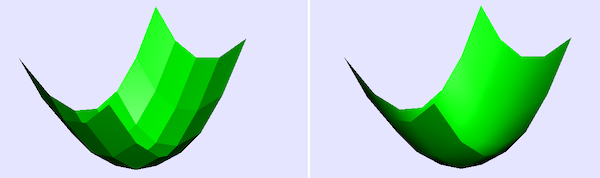
\includegraphics[bb=0 0 600 178 , width=8cm]{Cfig/nomal.png}

\hspace{35mm} perface \hspace{25mm} pervertex 

\vspace{\baselineskip}
\verb|topology| 修飾子は面の端の状態を指定する。指定がなければ、openとして処理される。

\vspace{\baselineskip}
 %%% /Users/hannya/Desktop/fig/table.tex 
%%% Generator=table.cdy 
{\unitlength=1cm%
\begin{picture}%
(13,8.4)(0,0)%
\special{pn 8}%
%
\special{pa     0 -3307}\special{pa     0    -0}%
\special{fp}%
\special{pa  1181 -3307}\special{pa  1181    -0}%
\special{fp}%
\special{pa  5118 -3307}\special{pa  5118    -0}%
\special{fp}%
\special{pa     0 -3307}\special{pa  5118 -3307}%
\special{fp}%
\special{pa     0 -2992}\special{pa  5118 -2992}%
\special{fp}%
\special{pa     0 -2362}\special{pa  5118 -2362}%
\special{fp}%
\special{pa     0 -1575}\special{pa  5118 -1575}%
\special{fp}%
\special{pa     0  -787}\special{pa  5118  -787}%
\special{fp}%
\special{pa     0    -0}\special{pa  5118    -0}%
\special{fp}%
\settowidth{\Width}{topology}\setlength{\Width}{-0.5\Width}%
\settoheight{\Height}{topology}\settodepth{\Depth}{topology}\setlength{\Height}{-0.5\Height}\setlength{\Depth}{0.5\Depth}\addtolength{\Height}{\Depth}%
\put(  1.500,  8.000){\hspace*{\Width}\raisebox{\Height}{topology}}%
%
\settowidth{\Width}{説明}\setlength{\Width}{-0.5\Width}%
\settoheight{\Height}{説明}\settodepth{\Depth}{説明}\setlength{\Height}{-0.5\Height}\setlength{\Depth}{0.5\Depth}\addtolength{\Height}{\Depth}%
\put(  8.000,  8.000){\hspace*{\Width}\raisebox{\Height}{説明}}%
%
\settowidth{\Width}{open}\setlength{\Width}{-0.5\Width}%
\settoheight{\Height}{open}\settodepth{\Depth}{open}\setlength{\Height}{-0.5\Height}\setlength{\Depth}{0.5\Depth}\addtolength{\Height}{\Depth}%
\put(  1.500,  6.800){\hspace*{\Width}\raisebox{\Height}{open}}%
%
\settowidth{\Width}{ \begin{minipage}{95mm}端点もしくは面の端の点までが面になる。その結果、(m-1)×(n-1)個の矩形ができる。 面は両サイドと1つの境界を持つ。 \end{minipage}}\setlength{\Width}{0\Width}%
\settoheight{\Height}{ \begin{minipage}{95mm}端点もしくは面の端の点までが面になる。その結果、(m-1)×(n-1)個の矩形ができる。 面は両サイドと1つの境界を持つ。 \end{minipage}}\settodepth{\Depth}{ \begin{minipage}{95mm}端点もしくは面の端の点までが面になる。その結果、(m-1)×(n-1)個の矩形ができる。 面は両サイドと1つの境界を持つ。 \end{minipage}}\setlength{\Height}{-0.5\Height}\setlength{\Depth}{0.5\Depth}\addtolength{\Height}{\Depth}%
\put(  3.050,  6.800){\hspace*{\Width}\raisebox{\Height}{ \begin{minipage}{95mm}端点もしくは面の端の点までが面になる。その結果、(m-1)×(n-1)個の矩形ができる。 面は両サイドと1つの境界を持つ。 \end{minipage}}}%
%
\settowidth{\Width}{closerows}\setlength{\Width}{-0.5\Width}%
\settoheight{\Height}{closerows}\settodepth{\Depth}{closerows}\setlength{\Height}{-0.5\Height}\setlength{\Depth}{0.5\Depth}\addtolength{\Height}{\Depth}%
\put(  1.500,  5.000){\hspace*{\Width}\raisebox{\Height}{closerows}}%
%
\settowidth{\Width}{ \begin{minipage}{95mm}各行の最初と最後の頂点が結合されて対応する面ができる。その結果、(m-1)×n 個の矩形ができる。面は両サイドと2つの境界を持つ。 \end{minipage}}\setlength{\Width}{0\Width}%
\settoheight{\Height}{ \begin{minipage}{95mm}各行の最初と最後の頂点が結合されて対応する面ができる。その結果、(m-1)×n 個の矩形ができる。面は両サイドと2つの境界を持つ。 \end{minipage}}\settodepth{\Depth}{ \begin{minipage}{95mm}各行の最初と最後の頂点が結合されて対応する面ができる。その結果、(m-1)×n 個の矩形ができる。面は両サイドと2つの境界を持つ。 \end{minipage}}\setlength{\Height}{-0.5\Height}\setlength{\Depth}{0.5\Depth}\addtolength{\Height}{\Depth}%
\put(  3.050,  5.000){\hspace*{\Width}\raisebox{\Height}{ \begin{minipage}{95mm}各行の最初と最後の頂点が結合されて対応する面ができる。その結果、(m-1)×n 個の矩形ができる。面は両サイドと2つの境界を持つ。 \end{minipage}}}%
%
\settowidth{\Width}{closecolumns}\setlength{\Width}{-0.5\Width}%
\settoheight{\Height}{closecolumns}\settodepth{\Depth}{closecolumns}\setlength{\Height}{-0.5\Height}\setlength{\Depth}{0.5\Depth}\addtolength{\Height}{\Depth}%
\put(  1.500,  3.000){\hspace*{\Width}\raisebox{\Height}{closecolumns}}%
%
\settowidth{\Width}{ \begin{minipage}{95mm}各列の最初と最後の頂点が結合されて対応する面ができる。その結果、m×(n-1) 個の矩形ができる。面は両サイドと2つの境界を持つ。  \end{minipage}}\setlength{\Width}{0\Width}%
\settoheight{\Height}{ \begin{minipage}{95mm}各列の最初と最後の頂点が結合されて対応する面ができる。その結果、m×(n-1) 個の矩形ができる。面は両サイドと2つの境界を持つ。  \end{minipage}}\settodepth{\Depth}{ \begin{minipage}{95mm}各列の最初と最後の頂点が結合されて対応する面ができる。その結果、m×(n-1) 個の矩形ができる。面は両サイドと2つの境界を持つ。  \end{minipage}}\setlength{\Height}{-0.5\Height}\setlength{\Depth}{0.5\Depth}\addtolength{\Height}{\Depth}%
\put(  3.050,  3.000){\hspace*{\Width}\raisebox{\Height}{ \begin{minipage}{95mm}各列の最初と最後の頂点が結合されて対応する面ができる。その結果、m×(n-1) 個の矩形ができる。面は両サイドと2つの境界を持つ。  \end{minipage}}}%
%
\settowidth{\Width}{closeboth}\setlength{\Width}{-0.5\Width}%
\settoheight{\Height}{closeboth}\settodepth{\Depth}{closeboth}\setlength{\Height}{-0.5\Height}\setlength{\Depth}{0.5\Depth}\addtolength{\Height}{\Depth}%
\put(  1.500,  1.000){\hspace*{\Width}\raisebox{\Height}{closeboth}}%
%
\settowidth{\Width}{ \begin{minipage}{95mm}各行の最初と最後および各列の最初と最後の頂点が結合されて対応する面ができる。その結果、m×n 個の矩形ができる。面は両サイドを持ち境界はない。 \end{minipage}}\setlength{\Width}{0\Width}%
\settoheight{\Height}{ \begin{minipage}{95mm}各行の最初と最後および各列の最初と最後の頂点が結合されて対応する面ができる。その結果、m×n 個の矩形ができる。面は両サイドを持ち境界はない。 \end{minipage}}\settodepth{\Depth}{ \begin{minipage}{95mm}各行の最初と最後および各列の最初と最後の頂点が結合されて対応する面ができる。その結果、m×n 個の矩形ができる。面は両サイドを持ち境界はない。 \end{minipage}}\setlength{\Height}{-0.5\Height}\setlength{\Depth}{0.5\Depth}\addtolength{\Height}{\Depth}%
\put(  3.050,  1.000){\hspace*{\Width}\raisebox{\Height}{ \begin{minipage}{95mm}各行の最初と最後および各列の最初と最後の頂点が結合されて対応する面ができる。その結果、m×n 個の矩形ができる。面は両サイドを持ち境界はない。 \end{minipage}}}%
%
\end{picture}}%

\hspace{20mm} 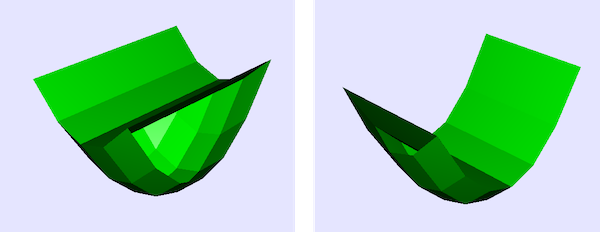
\includegraphics[bb=0 0 600 232 , width=8cm]{Cfig/topology.png}

\hspace{30mm} closerows \hspace{25mm} closecolumns 
 
\vspace{\baselineskip}
\noindent
{\bf 法線ベクトルを指定して網目を描く}:\verb|mesh3d(<int1>,<int2>,<list1>,<list2>)|

ユーザー定義による法線ベクトルによって網目を描く。

\verb|<int1>| 格子点の行数: m \verb|<int2>|:格子点の列数 n \verb|<list>|:格子点のリスト

\verb|<list2>| 各格子点での法線ベクトルのリスト。

リストの長さはいずれも m × n 。

\vspace{\baselineskip}
 %%% /Users/hannya/Desktop/fig/s0301tab.tex 
%%% Generator=s0301tab.cdy 
{\unitlength=1cm%
\begin{picture}%
(12.8,6)(0,0)%
\special{pn 8}%
%
\special{pa     0 -2362}\special{pa     0    -0}%
\special{fp}%
\special{pa   709 -2362}\special{pa   709    -0}%
\special{fp}%
\special{pa  2677 -2362}\special{pa  2677    -0}%
\special{fp}%
\special{pa  5039 -2362}\special{pa  5039    -0}%
\special{fp}%
\special{pa     0 -2362}\special{pa  5039 -2362}%
\special{fp}%
\special{pa     0 -2047}\special{pa  5039 -2047}%
\special{fp}%
\special{pa     0 -1260}\special{pa  5039 -1260}%
\special{fp}%
\special{pa     0  -945}\special{pa  5039  -945}%
\special{fp}%
\special{pa     0  -630}\special{pa  5039  -630}%
\special{fp}%
\special{pa     0  -315}\special{pa  5039  -315}%
\special{fp}%
\special{pa     0    -0}\special{pa  5039    -0}%
\special{fp}%
\settowidth{\Width}{修飾子}\setlength{\Width}{-0.5\Width}%
\settoheight{\Height}{修飾子}\settodepth{\Depth}{修飾子}\setlength{\Height}{-0.5\Height}\setlength{\Depth}{0.5\Depth}\addtolength{\Height}{\Depth}%
\put(  0.900,  5.600){\hspace*{\Width}\raisebox{\Height}{修飾子}}%
%
\settowidth{\Width}{値}\setlength{\Width}{-0.5\Width}%
\settoheight{\Height}{値}\settodepth{\Depth}{値}\setlength{\Height}{-0.5\Height}\setlength{\Depth}{0.5\Depth}\addtolength{\Height}{\Depth}%
\put(  4.300,  5.600){\hspace*{\Width}\raisebox{\Height}{値}}%
%
\settowidth{\Width}{効果}\setlength{\Width}{-0.5\Width}%
\settoheight{\Height}{効果}\settodepth{\Depth}{効果}\setlength{\Height}{-0.5\Height}\setlength{\Depth}{0.5\Depth}\addtolength{\Height}{\Depth}%
\put(  9.800,  5.600){\hspace*{\Width}\raisebox{\Height}{効果}}%
%
\settowidth{\Width}{topology}\setlength{\Width}{-0.5\Width}%
\settoheight{\Height}{topology}\settodepth{\Depth}{topology}\setlength{\Height}{-0.5\Height}\setlength{\Depth}{0.5\Depth}\addtolength{\Height}{\Depth}%
\put(  0.900,  4.200){\hspace*{\Width}\raisebox{\Height}{topology}}%
%
\settowidth{\Width}{<string>}\setlength{\Width}{-0.5\Width}%
\settoheight{\Height}{<string>}\settodepth{\Depth}{<string>}\setlength{\Height}{-0.5\Height}\setlength{\Depth}{0.5\Depth}\addtolength{\Height}{\Depth}%
\put(  4.300,  4.200){\hspace*{\Width}\raisebox{\Height}{<string>}}%
%
\settowidth{\Width}{ \begin{minipage}{70mm}topologyを指定する。\\値は open, closerows, closecolumns,\\ closeboth  のいずれか \end{minipage}}\setlength{\Width}{0\Width}%
\settoheight{\Height}{ \begin{minipage}{70mm}topologyを指定する。\\値は open, closerows, closecolumns,\\ closeboth  のいずれか \end{minipage}}\settodepth{\Depth}{ \begin{minipage}{70mm}topologyを指定する。\\値は open, closerows, closecolumns,\\ closeboth  のいずれか \end{minipage}}\setlength{\Height}{-0.5\Height}\setlength{\Depth}{0.5\Depth}\addtolength{\Height}{\Depth}%
\put(  6.850,  4.200){\hspace*{\Width}\raisebox{\Height}{ \begin{minipage}{70mm}topologyを指定する。\\値は open, closerows, closecolumns,\\ closeboth  のいずれか \end{minipage}}}%
%
\settowidth{\Width}{size}\setlength{\Width}{-0.5\Width}%
\settoheight{\Height}{size}\settodepth{\Depth}{size}\setlength{\Height}{-0.5\Height}\setlength{\Depth}{0.5\Depth}\addtolength{\Height}{\Depth}%
\put(  0.900,  2.800){\hspace*{\Width}\raisebox{\Height}{size}}%
%
\settowidth{\Width}{<real>}\setlength{\Width}{-0.5\Width}%
\settoheight{\Height}{<real>}\settodepth{\Depth}{<real>}\setlength{\Height}{-0.5\Height}\setlength{\Depth}{0.5\Depth}\addtolength{\Height}{\Depth}%
\put(  4.300,  2.800){\hspace*{\Width}\raisebox{\Height}{<real>}}%
%
\settowidth{\Width}{ 面の大きさを指定する}\setlength{\Width}{0\Width}%
\settoheight{\Height}{ 面の大きさを指定する}\settodepth{\Depth}{ 面の大きさを指定する}\setlength{\Height}{-0.5\Height}\setlength{\Depth}{0.5\Depth}\addtolength{\Height}{\Depth}%
\put(  6.850,  2.800){\hspace*{\Width}\raisebox{\Height}{ 面の大きさを指定する}}%
%
\settowidth{\Width}{color}\setlength{\Width}{-0.5\Width}%
\settoheight{\Height}{color}\settodepth{\Depth}{color}\setlength{\Height}{-0.5\Height}\setlength{\Depth}{0.5\Depth}\addtolength{\Height}{\Depth}%
\put(  0.900,  2.000){\hspace*{\Width}\raisebox{\Height}{color}}%
%
\settowidth{\Width}{[<real>,<real>,<real>]}\setlength{\Width}{-0.5\Width}%
\settoheight{\Height}{[<real>,<real>,<real>]}\settodepth{\Depth}{[<real>,<real>,<real>]}\setlength{\Height}{-0.5\Height}\setlength{\Depth}{0.5\Depth}\addtolength{\Height}{\Depth}%
\put(  4.300,  2.000){\hspace*{\Width}\raisebox{\Height}{[<real>,<real>,<real>]}}%
%
\settowidth{\Width}{ 色をRGBで指定する}\setlength{\Width}{0\Width}%
\settoheight{\Height}{ 色をRGBで指定する}\settodepth{\Depth}{ 色をRGBで指定する}\setlength{\Height}{-0.5\Height}\setlength{\Depth}{0.5\Depth}\addtolength{\Height}{\Depth}%
\put(  6.850,  2.000){\hspace*{\Width}\raisebox{\Height}{ 色をRGBで指定する}}%
%
\settowidth{\Width}{shininess}\setlength{\Width}{-0.5\Width}%
\settoheight{\Height}{shininess}\settodepth{\Depth}{shininess}\setlength{\Height}{-0.5\Height}\setlength{\Depth}{0.5\Depth}\addtolength{\Height}{\Depth}%
\put(  0.900,  1.200){\hspace*{\Width}\raisebox{\Height}{shininess}}%
%
\settowidth{\Width}{<real>}\setlength{\Width}{-0.5\Width}%
\settoheight{\Height}{<real>}\settodepth{\Depth}{<real>}\setlength{\Height}{-0.5\Height}\setlength{\Depth}{0.5\Depth}\addtolength{\Height}{\Depth}%
\put(  4.300,  1.200){\hspace*{\Width}\raisebox{\Height}{<real>}}%
%
\settowidth{\Width}{ 光沢を指定する}\setlength{\Width}{0\Width}%
\settoheight{\Height}{ 光沢を指定する}\settodepth{\Depth}{ 光沢を指定する}\setlength{\Height}{-0.5\Height}\setlength{\Depth}{0.5\Depth}\addtolength{\Height}{\Depth}%
\put(  6.850,  1.200){\hspace*{\Width}\raisebox{\Height}{ 光沢を指定する}}%
%
\settowidth{\Width}{alpha}\setlength{\Width}{-0.5\Width}%
\settoheight{\Height}{alpha}\settodepth{\Depth}{alpha}\setlength{\Height}{-0.5\Height}\setlength{\Depth}{0.5\Depth}\addtolength{\Height}{\Depth}%
\put(  0.900,  0.400){\hspace*{\Width}\raisebox{\Height}{alpha}}%
%
\settowidth{\Width}{<real>}\setlength{\Width}{-0.5\Width}%
\settoheight{\Height}{<real>}\settodepth{\Depth}{<real>}\setlength{\Height}{-0.5\Height}\setlength{\Depth}{0.5\Depth}\addtolength{\Height}{\Depth}%
\put(  4.300,  0.400){\hspace*{\Width}\raisebox{\Height}{<real>}}%
%
\settowidth{\Width}{ 透明度を指定する}\setlength{\Width}{0\Width}%
\settoheight{\Height}{ 透明度を指定する}\settodepth{\Depth}{ 透明度を指定する}\setlength{\Height}{-0.5\Height}\setlength{\Depth}{0.5\Depth}\addtolength{\Height}{\Depth}%
\put(  6.850,  0.400){\hspace*{\Width}\raisebox{\Height}{ 透明度を指定する}}%
%
\end{picture}}%

\subsection{光の当て方と表現}

\hypertarget{background3d}{}
\vspace{\baselineskip}
\noindent
{\bf 背景の色を設定する}:\verb|background3d(<colorvec>)|

背景の色 \verb|<colorvec>| をRGB値で設定する。

\hypertarget{lookat3d}{}
\vspace{\baselineskip}
\noindent
{\bf カメラの位置}:\verb|lookat3d(<point1>,<point2>,<vec>)|

3Dグラフィクスの表示は、空間に置いたカメラで物体を写していると考える。この関数は、カメラの位置と向きを設定する。カメラにはレンズがついていて、レンズの向き(視線の方向)で物を見ていると考える。

\verb|<point1>|:カメラの位置 \verb|<point2>|:回転の中心 \verb|<vec>|:視線の方向

\hypertarget{fieldofview3d}{}
\vspace{\baselineskip}
\noindent
{\bf 画角の設定 }:\verb|fieldofview3d(<real>)|

カメラの画角を設定する。実際のカメラの画角と同じ。画角が小さいと望遠(被写体が大きく写る)、大きいと広角(小さく写る)になる。初期設定は45°。

\hypertarget{depthrange3d}{}
\vspace{\baselineskip}
\noindent
{\bf カメラ深度の設定}:\verb|depthrange3d(<real1>,<real2>)|

カメラの最小・最大深度を設定する。カメラの深度とは、カメラ面(カメラを通り、視線方向に垂直な面)と点の距離。カメラ深度に入らないものは表示されない。第1引数が最小値、第2引数が最大値。

\hypertarget{renderhints3d}{}
\vspace{\baselineskip}
\noindent
{\bf レンダリングのヒントを設定する}:\verb|renderhints3d()|

レンダリングの過程における様々な比率のヒントを設定する。

\vspace{\baselineskip}
 %%% /Users/hannya/Desktop/fig/s0301tab.tex 
%%% Generator=s0301tab.cdy 
{\unitlength=1cm%
\begin{picture}%
(12.4,5.6)(0,0)%
\special{pn 8}%
%
\special{pa     0 -2205}\special{pa     0    -0}%
\special{fp}%
\special{pa   945 -2205}\special{pa   945    -0}%
\special{fp}%
\special{pa  1732 -2205}\special{pa  1732    -0}%
\special{fp}%
\special{pa  4882 -2205}\special{pa  4882    -0}%
\special{fp}%
\special{pa     0 -2205}\special{pa  4882 -2205}%
\special{fp}%
\special{pa     0 -1890}\special{pa  4882 -1890}%
\special{fp}%
\special{pa     0 -1575}\special{pa  4882 -1575}%
\special{fp}%
\special{pa     0  -945}\special{pa  4882  -945}%
\special{fp}%
\special{pa     0  -630}\special{pa  4882  -630}%
\special{fp}%
\special{pa     0    -0}\special{pa  4882    -0}%
\special{fp}%
\settowidth{\Width}{修飾子}\setlength{\Width}{-0.5\Width}%
\settoheight{\Height}{修飾子}\settodepth{\Depth}{修飾子}\setlength{\Height}{-0.5\Height}\setlength{\Depth}{0.5\Depth}\addtolength{\Height}{\Depth}%
\put(  1.200,  5.200){\hspace*{\Width}\raisebox{\Height}{修飾子}}%
%
\settowidth{\Width}{値}\setlength{\Width}{-0.5\Width}%
\settoheight{\Height}{値}\settodepth{\Depth}{値}\setlength{\Height}{-0.5\Height}\setlength{\Depth}{0.5\Depth}\addtolength{\Height}{\Depth}%
\put(  3.400,  5.200){\hspace*{\Width}\raisebox{\Height}{値}}%
%
\settowidth{\Width}{効果}\setlength{\Width}{-0.5\Width}%
\settoheight{\Height}{効果}\settodepth{\Depth}{効果}\setlength{\Height}{-0.5\Height}\setlength{\Depth}{0.5\Depth}\addtolength{\Height}{\Depth}%
\put(  8.400,  5.200){\hspace*{\Width}\raisebox{\Height}{効果}}%
%
\settowidth{\Width}{quality}\setlength{\Width}{-0.5\Width}%
\settoheight{\Height}{quality}\settodepth{\Depth}{quality}\setlength{\Height}{-0.5\Height}\setlength{\Depth}{0.5\Depth}\addtolength{\Height}{\Depth}%
\put(  1.200,  4.400){\hspace*{\Width}\raisebox{\Height}{quality}}%
%
\settowidth{\Width}{<int>}\setlength{\Width}{-0.5\Width}%
\settoheight{\Height}{<int>}\settodepth{\Depth}{<int>}\setlength{\Height}{-0.5\Height}\setlength{\Depth}{0.5\Depth}\addtolength{\Height}{\Depth}%
\put(  3.400,  4.400){\hspace*{\Width}\raisebox{\Height}{<int>}}%
%
\settowidth{\Width}{ 品質レベルを選ぶ。値は 0 以上 8 以下}\setlength{\Width}{0\Width}%
\settoheight{\Height}{ 品質レベルを選ぶ。値は 0 以上 8 以下}\settodepth{\Depth}{ 品質レベルを選ぶ。値は 0 以上 8 以下}\setlength{\Height}{-0.5\Height}\setlength{\Depth}{0.5\Depth}\addtolength{\Height}{\Depth}%
\put(  4.450,  4.400){\hspace*{\Width}\raisebox{\Height}{ 品質レベルを選ぶ。値は 0 以上 8 以下}}%
%
\settowidth{\Width}{renderMode}\setlength{\Width}{-0.5\Width}%
\settoheight{\Height}{renderMode}\settodepth{\Depth}{renderMode}\setlength{\Height}{-0.5\Height}\setlength{\Depth}{0.5\Depth}\addtolength{\Height}{\Depth}%
\put(  1.200,  3.200){\hspace*{\Width}\raisebox{\Height}{renderMode}}%
%
\settowidth{\Width}{<string>}\setlength{\Width}{-0.5\Width}%
\settoheight{\Height}{<string>}\settodepth{\Depth}{<string>}\setlength{\Height}{-0.5\Height}\setlength{\Depth}{0.5\Depth}\addtolength{\Height}{\Depth}%
\put(  3.400,  3.200){\hspace*{\Width}\raisebox{\Height}{<string>}}%
%
\settowidth{\Width}{ \begin{minipage}{80mm}レンダリングモードを指定する。\\値は "sinple" か "raycated" \end{minipage}}\setlength{\Width}{0\Width}%
\settoheight{\Height}{ \begin{minipage}{80mm}レンダリングモードを指定する。\\値は "sinple" か "raycated" \end{minipage}}\settodepth{\Depth}{ \begin{minipage}{80mm}レンダリングモードを指定する。\\値は "sinple" か "raycated" \end{minipage}}\setlength{\Height}{-0.5\Height}\setlength{\Depth}{0.5\Depth}\addtolength{\Height}{\Depth}%
\put(  4.450,  3.200){\hspace*{\Width}\raisebox{\Height}{ \begin{minipage}{80mm}レンダリングモードを指定する。\\値は "sinple" か "raycated" \end{minipage}}}%
%
\settowidth{\Width}{sampleRate}\setlength{\Width}{-0.5\Width}%
\settoheight{\Height}{sampleRate}\settodepth{\Depth}{sampleRate}\setlength{\Height}{-0.5\Height}\setlength{\Depth}{0.5\Depth}\addtolength{\Height}{\Depth}%
\put(  1.200,  2.000){\hspace*{\Width}\raisebox{\Height}{sampleRate}}%
%
\settowidth{\Width}{<int>}\setlength{\Width}{-0.5\Width}%
\settoheight{\Height}{<int>}\settodepth{\Depth}{<int>}\setlength{\Height}{-0.5\Height}\setlength{\Depth}{0.5\Depth}\addtolength{\Height}{\Depth}%
\put(  3.400,  2.000){\hspace*{\Width}\raisebox{\Height}{<int>}}%
%
\settowidth{\Width}{ ピクセルごとのサンプル数を設定。1以上の整数。}\setlength{\Width}{0\Width}%
\settoheight{\Height}{ ピクセルごとのサンプル数を設定。1以上の整数。}\settodepth{\Depth}{ ピクセルごとのサンプル数を設定。1以上の整数。}\setlength{\Height}{-0.5\Height}\setlength{\Depth}{0.5\Depth}\addtolength{\Height}{\Depth}%
\put(  4.450,  2.000){\hspace*{\Width}\raisebox{\Height}{ ピクセルごとのサンプル数を設定。1以上の整数。}}%
%
\settowidth{\Width}{screenError}\setlength{\Width}{-0.5\Width}%
\settoheight{\Height}{screenError}\settodepth{\Depth}{screenError}\setlength{\Height}{-0.5\Height}\setlength{\Depth}{0.5\Depth}\addtolength{\Height}{\Depth}%
\put(  1.200,  0.800){\hspace*{\Width}\raisebox{\Height}{screenError}}%
%
\settowidth{\Width}{<real>}\setlength{\Width}{-0.5\Width}%
\settoheight{\Height}{<real>}\settodepth{\Depth}{<real>}\setlength{\Height}{-0.5\Height}\setlength{\Depth}{0.5\Depth}\addtolength{\Height}{\Depth}%
\put(  3.400,  0.800){\hspace*{\Width}\raisebox{\Height}{<real>}}%
%
\settowidth{\Width}{ \begin{minipage}{70mm}ピクセルにおける最大の screen space error を設定する。値は 0より大きな実数 \end{minipage}}\setlength{\Width}{0\Width}%
\settoheight{\Height}{ \begin{minipage}{70mm}ピクセルにおける最大の screen space error を設定する。値は 0より大きな実数 \end{minipage}}\settodepth{\Depth}{ \begin{minipage}{70mm}ピクセルにおける最大の screen space error を設定する。値は 0より大きな実数 \end{minipage}}\setlength{\Height}{-0.5\Height}\setlength{\Depth}{0.5\Depth}\addtolength{\Height}{\Depth}%
\put(  4.450,  0.800){\hspace*{\Width}\raisebox{\Height}{ \begin{minipage}{70mm}ピクセルにおける最大の screen space error を設定する。値は 0より大きな実数 \end{minipage}}}%
%
\end{picture}}%

"quality" 修飾子は規定の品質レベルのいずれかを選ぶ。レベル 0 は最低の品質だが、最小のリソースですむ。最大の品質は 8 で、非常によい品質だが多くのリソースを必要とする。あらかじめ品質レベルが設定されているのは、個々のレンダリングヒントを操作することなく、全体の品質を簡単に管理できるようにするため。要請された品質レベルがサポートされない(例えばハードウェアの制限やリソースの制約のため)とき、Cindy3Dは下位のレベルに移行するかもしれない。

\vspace{\baselineskip}
\hspace{20mm} 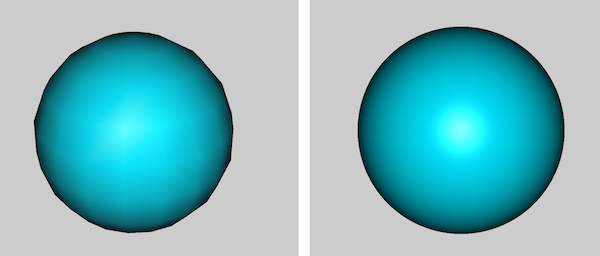
\includegraphics[bb=0 0 600 256 , width=8cm]{Cfig/render.png}

\hspace{30mm}\verb|quality->1| \hspace{20mm} \verb|quality->4|

\vspace{\baselineskip}
"renderMode" 修飾子は、オブジェクトのレンダリングについて指定する。"simple"の場合は、すべてのオブジェクトは三角形の網目としてレンダリングされる。このモードではシェーディングは頂点ごとに行われ、上図左のように粗削りになる。 "raycasted"の場合は、点・直線・球面はレイ・キャスティングを用いた連続面としてレンダリングされる。また、シェーディングは点ごとに行われる。上図右のようになる。 "raycasted" モードでは高品質が得られるがハードウェアの条件によっては時間がかかる。

"screenError" 修飾子は、スクリーン・スペース・エラーをデティール・アルゴリズムのレベルに設定する。 "simple" モードでは、 点・直線・球面は三角形の網目で近似される。最適化のために、小さい、あるいは遠いオブジェクトはレンダリング時間を節約するために少しの三角形網目にする。これを "level of detail"と呼ぶ。 Cindy3Dは、それぞれのプリミティブに対して、異なる三角形網目ごとに決められた定数を用いている。あるプリミティブに対しどの定数を用いるかは、各網目をスクリーン上に仮想的に投影し、ピクセルごとに最大の三角形の大きさを計測して決定される。それから、最大と予測される三角形サイズが「screenError」の下にある最も小さな網目が、プリミティブを生成するために使われる。これは、「screenError」の低い値がより高い品質となることを意味する。この修飾子は "raycasted"レンダリングモードのもとでは無効になる。

 "samplingRate" 修飾子は、オブジェクトのシルエットの滑らかさに影響する。サンプリング・レートは、出力イメージの各々のピクセルに対するサンプルの数を定める。最終的なピクセルの色はそれらのサンプルの平均値。サンプリングレートが高いほど、記憶領域と時間を消費するがオブジェクトシルエットはより滑らかになる。要請されたサンプリング・レートをサポートできないとき(例えばハードウェアの制限やリソースの制約のための)、Cindy3Dは低いサンプリング・レートに移行するかもしれない。

\vspace{\baselineskip}
※訳者の実験では、品質は quality の例で示した2通りくらいで、数値を変えてもあまり変化はなかった。(ハードウェアの制限などによるかもしれない)renderMode の ”simple” , ”raycasted” の違いも同様。あとの2つの修飾子の効果については翻訳時点では不明だった。デフォルトでは \verb|quality->1| なので、 \verb|renderhints3d(quality->4)| もしくは \verb|renderhints3d(renderMode->"raycasted")| で運用するのがよさそうだ。

\hypertarget{pointlight3d}{} 
\vspace{\baselineskip}
\noindent
{\bf 点光源の設定}:\verb|pointlight3d(<int>)|

\verb|<int>| は,光源の番号で0以上7以下の整数。

点光源を発生または修正する。指定された光源がすでに存在するならば修飾子によって指定された状態に修正し、利用可能にする。そうでなければ、指定された点光源を作る。修飾子がなければ初期値が使われる。点光源は8つまで作ることができ、それぞれに番号を振る。

\vspace{\baselineskip}
 %%% /Users/hannya/Desktop/fig/s0301tab.tex 
%%% Generator=s0301tab.cdy 
{\unitlength=1cm%
\begin{picture}%
(13.2,8.4)(0,0)%
\special{pn 8}%
%
\special{pa     0 -3307}\special{pa     0    -0}%
\special{fp}%
\special{pa   945 -3307}\special{pa   945    -0}%
\special{fp}%
\special{pa  2047 -3307}\special{pa  2047    -0}%
\special{fp}%
\special{pa  5197 -3307}\special{pa  5197    -0}%
\special{fp}%
\special{pa     0 -3307}\special{pa  5197 -3307}%
\special{fp}%
\special{pa     0 -2992}\special{pa  5197 -2992}%
\special{fp}%
\special{pa     0 -2362}\special{pa  5197 -2362}%
\special{fp}%
\special{pa     0 -1732}\special{pa  5197 -1732}%
\special{fp}%
\special{pa     0 -1102}\special{pa  5197 -1102}%
\special{fp}%
\special{pa     0  -787}\special{pa  5197  -787}%
\special{fp}%
\special{pa     0    -0}\special{pa  5197    -0}%
\special{fp}%
\settowidth{\Width}{修飾子}\setlength{\Width}{-0.5\Width}%
\settoheight{\Height}{修飾子}\settodepth{\Depth}{修飾子}\setlength{\Height}{-0.5\Height}\setlength{\Depth}{0.5\Depth}\addtolength{\Height}{\Depth}%
\put(  1.200,  8.000){\hspace*{\Width}\raisebox{\Height}{修飾子}}%
%
\settowidth{\Width}{値}\setlength{\Width}{-0.5\Width}%
\settoheight{\Height}{値}\settodepth{\Depth}{値}\setlength{\Height}{-0.5\Height}\setlength{\Depth}{0.5\Depth}\addtolength{\Height}{\Depth}%
\put(  3.800,  8.000){\hspace*{\Width}\raisebox{\Height}{値}}%
%
\settowidth{\Width}{効果}\setlength{\Width}{-0.5\Width}%
\settoheight{\Height}{効果}\settodepth{\Depth}{効果}\setlength{\Height}{-0.5\Height}\setlength{\Depth}{0.5\Depth}\addtolength{\Height}{\Depth}%
\put(  9.200,  8.000){\hspace*{\Width}\raisebox{\Height}{効果}}%
%
\settowidth{\Width}{ambient}\setlength{\Width}{-0.5\Width}%
\settoheight{\Height}{ambient}\settodepth{\Depth}{ambient}\setlength{\Height}{-0.5\Height}\setlength{\Depth}{0.5\Depth}\addtolength{\Height}{\Depth}%
\put(  1.200,  6.800){\hspace*{\Width}\raisebox{\Height}{ambient}}%
%
\settowidth{\Width}{[R,G,B]}\setlength{\Width}{-0.5\Width}%
\settoheight{\Height}{[R,G,B]}\settodepth{\Depth}{[R,G,B]}\setlength{\Height}{-0.5\Height}\setlength{\Depth}{0.5\Depth}\addtolength{\Height}{\Depth}%
\put(  3.800,  6.800){\hspace*{\Width}\raisebox{\Height}{[R,G,B]}}%
%
\settowidth{\Width}{ \begin{minipage}{80mm}周囲の色をRGB 値で指定された色にする\\ (初期値は [0,0,0]) \end{minipage}}\setlength{\Width}{0\Width}%
\settoheight{\Height}{ \begin{minipage}{80mm}周囲の色をRGB 値で指定された色にする\\ (初期値は [0,0,0]) \end{minipage}}\settodepth{\Depth}{ \begin{minipage}{80mm}周囲の色をRGB 値で指定された色にする\\ (初期値は [0,0,0]) \end{minipage}}\setlength{\Height}{-0.5\Height}\setlength{\Depth}{0.5\Depth}\addtolength{\Height}{\Depth}%
\put(  5.250,  6.800){\hspace*{\Width}\raisebox{\Height}{ \begin{minipage}{80mm}周囲の色をRGB 値で指定された色にする\\ (初期値は [0,0,0]) \end{minipage}}}%
%
\settowidth{\Width}{diffuse}\setlength{\Width}{-0.5\Width}%
\settoheight{\Height}{diffuse}\settodepth{\Depth}{diffuse}\setlength{\Height}{-0.5\Height}\setlength{\Depth}{0.5\Depth}\addtolength{\Height}{\Depth}%
\put(  1.200,  5.200){\hspace*{\Width}\raisebox{\Height}{diffuse}}%
%
\settowidth{\Width}{[R,G,B]}\setlength{\Width}{-0.5\Width}%
\settoheight{\Height}{[R,G,B]}\settodepth{\Depth}{[R,G,B]}\setlength{\Height}{-0.5\Height}\setlength{\Depth}{0.5\Depth}\addtolength{\Height}{\Depth}%
\put(  3.800,  5.200){\hspace*{\Width}\raisebox{\Height}{[R,G,B]}}%
%
\settowidth{\Width}{ \begin{minipage}{80mm}拡散する光の色を RGB 値で指定された色にする\\ (初期値は [1,1,1]) \end{minipage}}\setlength{\Width}{0\Width}%
\settoheight{\Height}{ \begin{minipage}{80mm}拡散する光の色を RGB 値で指定された色にする\\ (初期値は [1,1,1]) \end{minipage}}\settodepth{\Depth}{ \begin{minipage}{80mm}拡散する光の色を RGB 値で指定された色にする\\ (初期値は [1,1,1]) \end{minipage}}\setlength{\Height}{-0.5\Height}\setlength{\Depth}{0.5\Depth}\addtolength{\Height}{\Depth}%
\put(  5.250,  5.200){\hspace*{\Width}\raisebox{\Height}{ \begin{minipage}{80mm}拡散する光の色を RGB 値で指定された色にする\\ (初期値は [1,1,1]) \end{minipage}}}%
%
\settowidth{\Width}{specular}\setlength{\Width}{-0.5\Width}%
\settoheight{\Height}{specular}\settodepth{\Depth}{specular}\setlength{\Height}{-0.5\Height}\setlength{\Depth}{0.5\Depth}\addtolength{\Height}{\Depth}%
\put(  1.200,  3.600){\hspace*{\Width}\raisebox{\Height}{specular}}%
%
\settowidth{\Width}{[R,G,B]}\setlength{\Width}{-0.5\Width}%
\settoheight{\Height}{[R,G,B]}\settodepth{\Depth}{[R,G,B]}\setlength{\Height}{-0.5\Height}\setlength{\Depth}{0.5\Depth}\addtolength{\Height}{\Depth}%
\put(  3.800,  3.600){\hspace*{\Width}\raisebox{\Height}{[R,G,B]}}%
%
\settowidth{\Width}{ \begin{minipage}{70mm}反射光の色を RGB 値で指定された色にする\\ (初期値は [1,1,1]) \end{minipage}}\setlength{\Width}{0\Width}%
\settoheight{\Height}{ \begin{minipage}{70mm}反射光の色を RGB 値で指定された色にする\\ (初期値は [1,1,1]) \end{minipage}}\settodepth{\Depth}{ \begin{minipage}{70mm}反射光の色を RGB 値で指定された色にする\\ (初期値は [1,1,1]) \end{minipage}}\setlength{\Height}{-0.5\Height}\setlength{\Depth}{0.5\Depth}\addtolength{\Height}{\Depth}%
\put(  5.250,  3.600){\hspace*{\Width}\raisebox{\Height}{ \begin{minipage}{70mm}反射光の色を RGB 値で指定された色にする\\ (初期値は [1,1,1]) \end{minipage}}}%
%
\settowidth{\Width}{position}\setlength{\Width}{-0.5\Width}%
\settoheight{\Height}{position}\settodepth{\Depth}{position}\setlength{\Height}{-0.5\Height}\setlength{\Depth}{0.5\Depth}\addtolength{\Height}{\Depth}%
\put(  1.200,  2.400){\hspace*{\Width}\raisebox{\Height}{position}}%
%
\settowidth{\Width}{<point>}\setlength{\Width}{-0.5\Width}%
\settoheight{\Height}{<point>}\settodepth{\Depth}{<point>}\setlength{\Height}{-0.5\Height}\setlength{\Depth}{0.5\Depth}\addtolength{\Height}{\Depth}%
\put(  3.800,  2.400){\hspace*{\Width}\raisebox{\Height}{<point>}}%
%
\settowidth{\Width}{点の位置 (初期値は [0,0,0])}\setlength{\Width}{0\Width}%
\settoheight{\Height}{点の位置 (初期値は [0,0,0])}\settodepth{\Depth}{点の位置 (初期値は [0,0,0])}\setlength{\Height}{-0.5\Height}\setlength{\Depth}{0.5\Depth}\addtolength{\Height}{\Depth}%
\put(  5.250,  2.400){\hspace*{\Width}\raisebox{\Height}{点の位置 (初期値は [0,0,0])}}%
%
\settowidth{\Width}{frame}\setlength{\Width}{-0.5\Width}%
\settoheight{\Height}{frame}\settodepth{\Depth}{frame}\setlength{\Height}{-0.5\Height}\setlength{\Depth}{0.5\Depth}\addtolength{\Height}{\Depth}%
\put(  1.200,  1.000){\hspace*{\Width}\raisebox{\Height}{frame}}%
%
\settowidth{\Width}{<string>}\setlength{\Width}{-0.5\Width}%
\settoheight{\Height}{<string>}\settodepth{\Depth}{<string>}\setlength{\Height}{-0.5\Height}\setlength{\Depth}{0.5\Depth}\addtolength{\Height}{\Depth}%
\put(  3.800,  1.000){\hspace*{\Width}\raisebox{\Height}{<string>}}%
%
\settowidth{\Width}{ \begin{minipage}{70mm}位置がカメラフレームに依存するか、絶対位置かを指定する。値は"camera" か "world" で、初期値は "camera" \end{minipage}}\setlength{\Width}{0\Width}%
\settoheight{\Height}{ \begin{minipage}{70mm}位置がカメラフレームに依存するか、絶対位置かを指定する。値は"camera" か "world" で、初期値は "camera" \end{minipage}}\settodepth{\Depth}{ \begin{minipage}{70mm}位置がカメラフレームに依存するか、絶対位置かを指定する。値は"camera" か "world" で、初期値は "camera" \end{minipage}}\setlength{\Height}{-0.5\Height}\setlength{\Depth}{0.5\Depth}\addtolength{\Height}{\Depth}%
\put(  5.250,  1.000){\hspace*{\Width}\raisebox{\Height}{ \begin{minipage}{70mm}位置がカメラフレームに依存するか、絶対位置かを指定する。値は"camera" か "world" で、初期値は "camera" \end{minipage}}}%
%
\end{picture}}%

\vspace{\baselineskip}
\hspace{15mm} 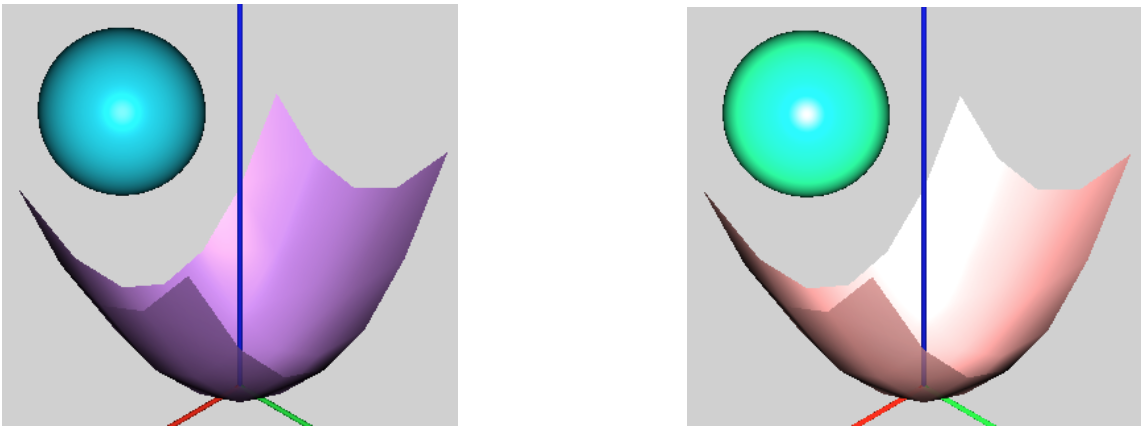
\includegraphics[bb=0 0 572 216 , width=10cm]{Cfig/light1.png}

\hspace{25mm}点光源の指定なし \hspace{20mm} 点光源1 \verb|diffuse->[1,1,0]|

\vspace{\baselineskip}
\hspace{15mm} 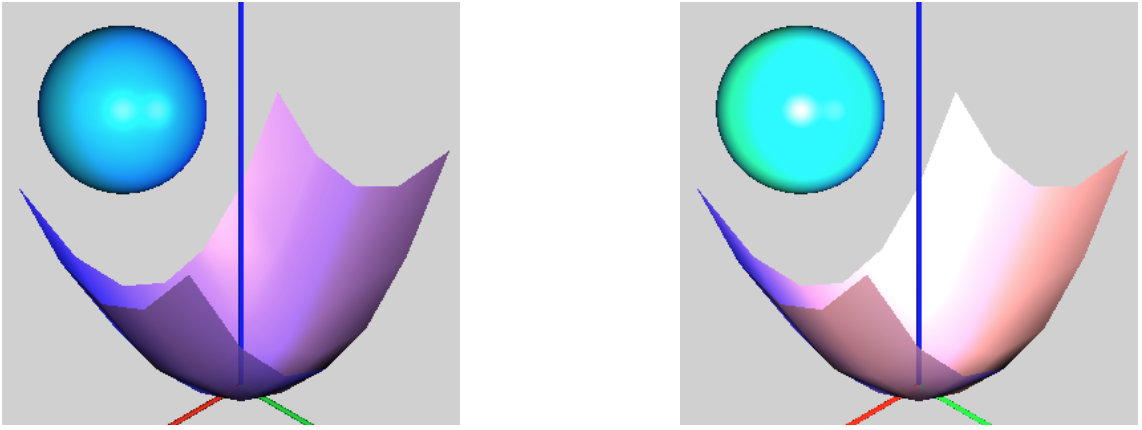
\includegraphics[bb=0 0 572 215 , width=10cm]{Cfig/light2.png}

\hspace{5mm}点光源2 \verb|position->[8,0,0],diffuse->[0,0,1])| \hspace{5mm} 点光源1と2

\hypertarget{directionallight3d}{}
\vspace{\baselineskip}
\noindent
{\bf 方向光源の設定}:\verb|directionallight3d(<int>)|

\verb|<int>|は,方向光源の番号で0以上7以下の整数。

方向光源を発生または修正する。 指定された方向光源がすでに存在するならば修飾子によって指定された状態に修正し、利用可能にする。そうでなければ、指定された方向光源を作る。修飾子がなければ初期値が使われる。

\vspace{\baselineskip}
 %%% /Users/hannya/Desktop/fig/s0301tab.tex 
%%% Generator=s0301tab.cdy 
{\unitlength=1cm%
\begin{picture}%
(13.2,8.4)(0,0)%
\special{pn 8}%
%
\special{pa     0 -3307}\special{pa     0    -0}%
\special{fp}%
\special{pa   945 -3307}\special{pa   945    -0}%
\special{fp}%
\special{pa  2047 -3307}\special{pa  2047    -0}%
\special{fp}%
\special{pa  5197 -3307}\special{pa  5197    -0}%
\special{fp}%
\special{pa     0 -3307}\special{pa  5197 -3307}%
\special{fp}%
\special{pa     0 -2992}\special{pa  5197 -2992}%
\special{fp}%
\special{pa     0 -2362}\special{pa  5197 -2362}%
\special{fp}%
\special{pa     0 -1732}\special{pa  5197 -1732}%
\special{fp}%
\special{pa     0 -1102}\special{pa  5197 -1102}%
\special{fp}%
\special{pa     0  -787}\special{pa  5197  -787}%
\special{fp}%
\special{pa     0    -0}\special{pa  5197    -0}%
\special{fp}%
\settowidth{\Width}{修飾子}\setlength{\Width}{-0.5\Width}%
\settoheight{\Height}{修飾子}\settodepth{\Depth}{修飾子}\setlength{\Height}{-0.5\Height}\setlength{\Depth}{0.5\Depth}\addtolength{\Height}{\Depth}%
\put(  1.200,  8.000){\hspace*{\Width}\raisebox{\Height}{修飾子}}%
%
\settowidth{\Width}{値}\setlength{\Width}{-0.5\Width}%
\settoheight{\Height}{値}\settodepth{\Depth}{値}\setlength{\Height}{-0.5\Height}\setlength{\Depth}{0.5\Depth}\addtolength{\Height}{\Depth}%
\put(  3.800,  8.000){\hspace*{\Width}\raisebox{\Height}{値}}%
%
\settowidth{\Width}{効果}\setlength{\Width}{-0.5\Width}%
\settoheight{\Height}{効果}\settodepth{\Depth}{効果}\setlength{\Height}{-0.5\Height}\setlength{\Depth}{0.5\Depth}\addtolength{\Height}{\Depth}%
\put(  9.200,  8.000){\hspace*{\Width}\raisebox{\Height}{効果}}%
%
\settowidth{\Width}{ambient}\setlength{\Width}{-0.5\Width}%
\settoheight{\Height}{ambient}\settodepth{\Depth}{ambient}\setlength{\Height}{-0.5\Height}\setlength{\Depth}{0.5\Depth}\addtolength{\Height}{\Depth}%
\put(  1.200,  6.800){\hspace*{\Width}\raisebox{\Height}{ambient}}%
%
\settowidth{\Width}{[R,G,B]}\setlength{\Width}{-0.5\Width}%
\settoheight{\Height}{[R,G,B]}\settodepth{\Depth}{[R,G,B]}\setlength{\Height}{-0.5\Height}\setlength{\Depth}{0.5\Depth}\addtolength{\Height}{\Depth}%
\put(  3.800,  6.800){\hspace*{\Width}\raisebox{\Height}{[R,G,B]}}%
%
\settowidth{\Width}{ \begin{minipage}{80mm}周囲の色をRGB 値で指定された色にする\\ (初期値は [0,0,0]) \end{minipage}}\setlength{\Width}{0\Width}%
\settoheight{\Height}{ \begin{minipage}{80mm}周囲の色をRGB 値で指定された色にする\\ (初期値は [0,0,0]) \end{minipage}}\settodepth{\Depth}{ \begin{minipage}{80mm}周囲の色をRGB 値で指定された色にする\\ (初期値は [0,0,0]) \end{minipage}}\setlength{\Height}{-0.5\Height}\setlength{\Depth}{0.5\Depth}\addtolength{\Height}{\Depth}%
\put(  5.250,  6.800){\hspace*{\Width}\raisebox{\Height}{ \begin{minipage}{80mm}周囲の色をRGB 値で指定された色にする\\ (初期値は [0,0,0]) \end{minipage}}}%
%
\settowidth{\Width}{diffuse}\setlength{\Width}{-0.5\Width}%
\settoheight{\Height}{diffuse}\settodepth{\Depth}{diffuse}\setlength{\Height}{-0.5\Height}\setlength{\Depth}{0.5\Depth}\addtolength{\Height}{\Depth}%
\put(  1.200,  5.200){\hspace*{\Width}\raisebox{\Height}{diffuse}}%
%
\settowidth{\Width}{[R,G,B]}\setlength{\Width}{-0.5\Width}%
\settoheight{\Height}{[R,G,B]}\settodepth{\Depth}{[R,G,B]}\setlength{\Height}{-0.5\Height}\setlength{\Depth}{0.5\Depth}\addtolength{\Height}{\Depth}%
\put(  3.800,  5.200){\hspace*{\Width}\raisebox{\Height}{[R,G,B]}}%
%
\settowidth{\Width}{ \begin{minipage}{80mm}拡散する光の色を RGB 値で指定された色にする\\ (初期値は [1,1,1]) \end{minipage}}\setlength{\Width}{0\Width}%
\settoheight{\Height}{ \begin{minipage}{80mm}拡散する光の色を RGB 値で指定された色にする\\ (初期値は [1,1,1]) \end{minipage}}\settodepth{\Depth}{ \begin{minipage}{80mm}拡散する光の色を RGB 値で指定された色にする\\ (初期値は [1,1,1]) \end{minipage}}\setlength{\Height}{-0.5\Height}\setlength{\Depth}{0.5\Depth}\addtolength{\Height}{\Depth}%
\put(  5.250,  5.200){\hspace*{\Width}\raisebox{\Height}{ \begin{minipage}{80mm}拡散する光の色を RGB 値で指定された色にする\\ (初期値は [1,1,1]) \end{minipage}}}%
%
\settowidth{\Width}{specular}\setlength{\Width}{-0.5\Width}%
\settoheight{\Height}{specular}\settodepth{\Depth}{specular}\setlength{\Height}{-0.5\Height}\setlength{\Depth}{0.5\Depth}\addtolength{\Height}{\Depth}%
\put(  1.200,  3.600){\hspace*{\Width}\raisebox{\Height}{specular}}%
%
\settowidth{\Width}{[R,G,B]}\setlength{\Width}{-0.5\Width}%
\settoheight{\Height}{[R,G,B]}\settodepth{\Depth}{[R,G,B]}\setlength{\Height}{-0.5\Height}\setlength{\Depth}{0.5\Depth}\addtolength{\Height}{\Depth}%
\put(  3.800,  3.600){\hspace*{\Width}\raisebox{\Height}{[R,G,B]}}%
%
\settowidth{\Width}{ \begin{minipage}{70mm}反射光の色を RGB 値で指定された色にする\\ (初期値は [1,1,1]) \end{minipage}}\setlength{\Width}{0\Width}%
\settoheight{\Height}{ \begin{minipage}{70mm}反射光の色を RGB 値で指定された色にする\\ (初期値は [1,1,1]) \end{minipage}}\settodepth{\Depth}{ \begin{minipage}{70mm}反射光の色を RGB 値で指定された色にする\\ (初期値は [1,1,1]) \end{minipage}}\setlength{\Height}{-0.5\Height}\setlength{\Depth}{0.5\Depth}\addtolength{\Height}{\Depth}%
\put(  5.250,  3.600){\hspace*{\Width}\raisebox{\Height}{ \begin{minipage}{70mm}反射光の色を RGB 値で指定された色にする\\ (初期値は [1,1,1]) \end{minipage}}}%
%
\settowidth{\Width}{direction}\setlength{\Width}{-0.5\Width}%
\settoheight{\Height}{direction}\settodepth{\Depth}{direction}\setlength{\Height}{-0.5\Height}\setlength{\Depth}{0.5\Depth}\addtolength{\Height}{\Depth}%
\put(  1.200,  2.400){\hspace*{\Width}\raisebox{\Height}{direction}}%
%
\settowidth{\Width}{<vec>}\setlength{\Width}{-0.5\Width}%
\settoheight{\Height}{<vec>}\settodepth{\Depth}{<vec>}\setlength{\Height}{-0.5\Height}\setlength{\Depth}{0.5\Depth}\addtolength{\Height}{\Depth}%
\put(  3.800,  2.400){\hspace*{\Width}\raisebox{\Height}{<vec>}}%
%
\settowidth{\Width}{ 光の方向 (初期値は [0,-1,0])}\setlength{\Width}{0\Width}%
\settoheight{\Height}{ 光の方向 (初期値は [0,-1,0])}\settodepth{\Depth}{ 光の方向 (初期値は [0,-1,0])}\setlength{\Height}{-0.5\Height}\setlength{\Depth}{0.5\Depth}\addtolength{\Height}{\Depth}%
\put(  5.250,  2.400){\hspace*{\Width}\raisebox{\Height}{ 光の方向 (初期値は [0,-1,0])}}%
%
\settowidth{\Width}{frame}\setlength{\Width}{-0.5\Width}%
\settoheight{\Height}{frame}\settodepth{\Depth}{frame}\setlength{\Height}{-0.5\Height}\setlength{\Depth}{0.5\Depth}\addtolength{\Height}{\Depth}%
\put(  1.200,  1.000){\hspace*{\Width}\raisebox{\Height}{frame}}%
%
\settowidth{\Width}{<string>}\setlength{\Width}{-0.5\Width}%
\settoheight{\Height}{<string>}\settodepth{\Depth}{<string>}\setlength{\Height}{-0.5\Height}\setlength{\Depth}{0.5\Depth}\addtolength{\Height}{\Depth}%
\put(  3.800,  1.000){\hspace*{\Width}\raisebox{\Height}{<string>}}%
%
\settowidth{\Width}{ \begin{minipage}{70mm}方向がカメラフレームに依存するか、絶対的かを指定する。値は"camera" か "world" で、初期値は "camera" \end{minipage}}\setlength{\Width}{0\Width}%
\settoheight{\Height}{ \begin{minipage}{70mm}方向がカメラフレームに依存するか、絶対的かを指定する。値は"camera" か "world" で、初期値は "camera" \end{minipage}}\settodepth{\Depth}{ \begin{minipage}{70mm}方向がカメラフレームに依存するか、絶対的かを指定する。値は"camera" か "world" で、初期値は "camera" \end{minipage}}\setlength{\Height}{-0.5\Height}\setlength{\Depth}{0.5\Depth}\addtolength{\Height}{\Depth}%
\put(  5.250,  1.000){\hspace*{\Width}\raisebox{\Height}{ \begin{minipage}{70mm}方向がカメラフレームに依存するか、絶対的かを指定する。値は"camera" か "world" で、初期値は "camera" \end{minipage}}}%
%
\end{picture}}%

\vspace{\baselineskip}
\hspace{15mm} 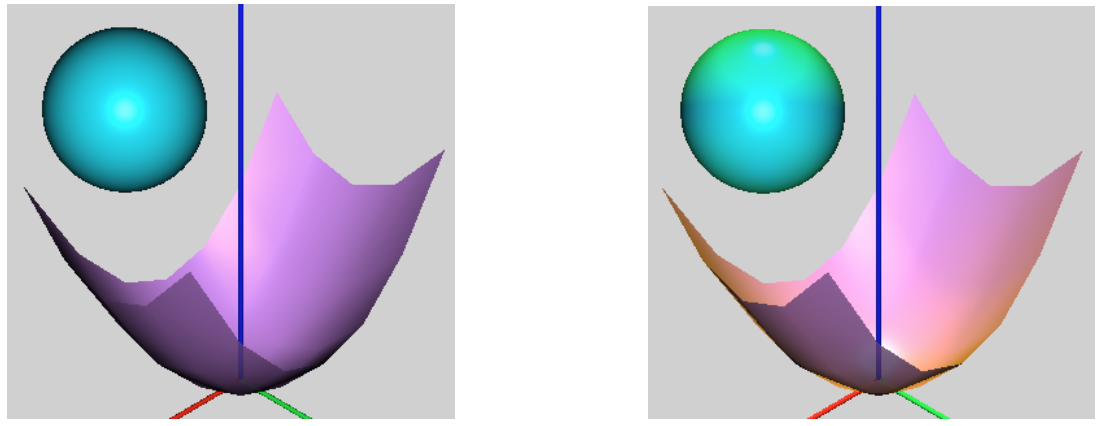
\includegraphics[bb=0 0 549 213 , width=10cm]{Cfig/direclight1.png}

\hspace{20mm}方向光源の指定なし \hspace{20mm} 方向光源1 \verb|diffuse->[1,1,0]|

\vspace{\baselineskip}
\hspace{15mm} 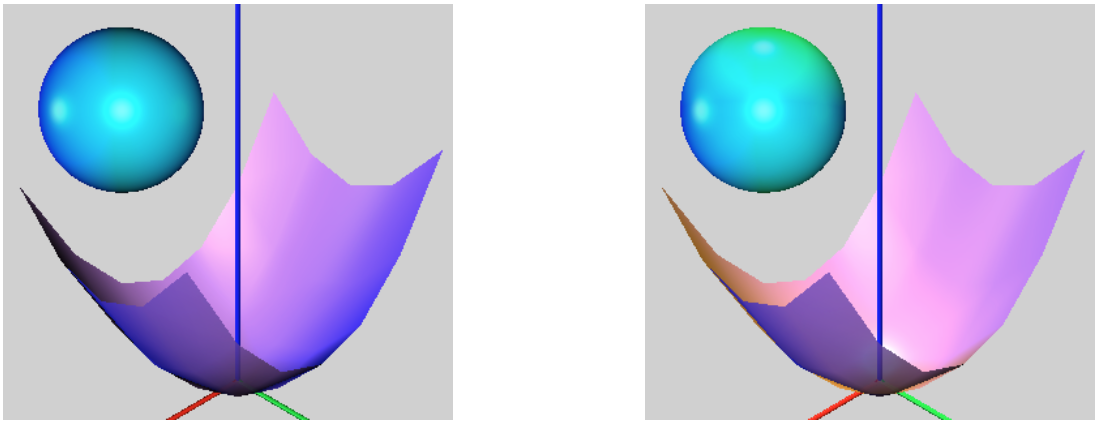
\includegraphics[bb=0 0 550 214 , width=10cm]{Cfig/direclight2.png}

\hspace{2mm}方向光源2 \verb|direction->[8,0,0],diffuse->[0,0,1])| \hspace{5mm} 方向光源1と2

\hypertarget{spotlight3d}{} 
\vspace{\baselineskip}
\noindent
{\bf スポットライトの設定}:\verb|spotlight3d(<int>)|

\verb|<int>|は,光源の番号で0以上7以下の整数。

スポットライトを発生または修正する。 指定された光源がすでに存在するならば修飾子によって指定された状態に修正し、利用可能にする。そうでなければ、指定された光源を作る。修飾子がなければ初期値が使われる。

\vspace{\baselineskip}
 %%% /Users/hannya/Desktop/fig/s0301tab.tex 
%%% Generator=s0301tab.cdy 
{\unitlength=1cm%
\begin{picture}%
(13.2,11.8)(0,0)%
\special{pn 8}%
%
\special{pa     0 -4646}\special{pa     0    -0}%
\special{fp}%
\special{pa   945 -4646}\special{pa   945    -0}%
\special{fp}%
\special{pa  2047 -4646}\special{pa  2047    -0}%
\special{fp}%
\special{pa  5197 -4646}\special{pa  5197    -0}%
\special{fp}%
\special{pa     0 -4646}\special{pa  5197 -4646}%
\special{fp}%
\special{pa     0 -4331}\special{pa  5197 -4331}%
\special{fp}%
\special{pa     0 -3701}\special{pa  5197 -3701}%
\special{fp}%
\special{pa     0 -3071}\special{pa  5197 -3071}%
\special{fp}%
\special{pa     0 -2441}\special{pa  5197 -2441}%
\special{fp}%
\special{pa     0 -2126}\special{pa  5197 -2126}%
\special{fp}%
\special{pa     0 -1811}\special{pa  5197 -1811}%
\special{fp}%
\special{pa     0 -1102}\special{pa  5197 -1102}%
\special{fp}%
\special{pa     0  -787}\special{pa  5197  -787}%
\special{fp}%
\special{pa     0    -0}\special{pa  5197    -0}%
\special{fp}%
\settowidth{\Width}{修飾子}\setlength{\Width}{-0.5\Width}%
\settoheight{\Height}{修飾子}\settodepth{\Depth}{修飾子}\setlength{\Height}{-0.5\Height}\setlength{\Depth}{0.5\Depth}\addtolength{\Height}{\Depth}%
\put(  1.200, 11.400){\hspace*{\Width}\raisebox{\Height}{修飾子}}%
%
\settowidth{\Width}{値}\setlength{\Width}{-0.5\Width}%
\settoheight{\Height}{値}\settodepth{\Depth}{値}\setlength{\Height}{-0.5\Height}\setlength{\Depth}{0.5\Depth}\addtolength{\Height}{\Depth}%
\put(  3.800, 11.400){\hspace*{\Width}\raisebox{\Height}{値}}%
%
\settowidth{\Width}{効果}\setlength{\Width}{-0.5\Width}%
\settoheight{\Height}{効果}\settodepth{\Depth}{効果}\setlength{\Height}{-0.5\Height}\setlength{\Depth}{0.5\Depth}\addtolength{\Height}{\Depth}%
\put(  9.200, 11.400){\hspace*{\Width}\raisebox{\Height}{効果}}%
%
\settowidth{\Width}{ambient}\setlength{\Width}{-0.5\Width}%
\settoheight{\Height}{ambient}\settodepth{\Depth}{ambient}\setlength{\Height}{-0.5\Height}\setlength{\Depth}{0.5\Depth}\addtolength{\Height}{\Depth}%
\put(  1.200, 10.200){\hspace*{\Width}\raisebox{\Height}{ambient}}%
%
\settowidth{\Width}{[R,G,B]}\setlength{\Width}{-0.5\Width}%
\settoheight{\Height}{[R,G,B]}\settodepth{\Depth}{[R,G,B]}\setlength{\Height}{-0.5\Height}\setlength{\Depth}{0.5\Depth}\addtolength{\Height}{\Depth}%
\put(  3.800, 10.200){\hspace*{\Width}\raisebox{\Height}{[R,G,B]}}%
%
\settowidth{\Width}{ \begin{minipage}{80mm}周囲の色をRGB 値で指定された色にする\\ (初期値は [0,0,0]) \end{minipage}}\setlength{\Width}{0\Width}%
\settoheight{\Height}{ \begin{minipage}{80mm}周囲の色をRGB 値で指定された色にする\\ (初期値は [0,0,0]) \end{minipage}}\settodepth{\Depth}{ \begin{minipage}{80mm}周囲の色をRGB 値で指定された色にする\\ (初期値は [0,0,0]) \end{minipage}}\setlength{\Height}{-0.5\Height}\setlength{\Depth}{0.5\Depth}\addtolength{\Height}{\Depth}%
\put(  5.250, 10.200){\hspace*{\Width}\raisebox{\Height}{ \begin{minipage}{80mm}周囲の色をRGB 値で指定された色にする\\ (初期値は [0,0,0]) \end{minipage}}}%
%
\settowidth{\Width}{diffuse}\setlength{\Width}{-0.5\Width}%
\settoheight{\Height}{diffuse}\settodepth{\Depth}{diffuse}\setlength{\Height}{-0.5\Height}\setlength{\Depth}{0.5\Depth}\addtolength{\Height}{\Depth}%
\put(  1.200,  8.600){\hspace*{\Width}\raisebox{\Height}{diffuse}}%
%
\settowidth{\Width}{[R,G,B]}\setlength{\Width}{-0.5\Width}%
\settoheight{\Height}{[R,G,B]}\settodepth{\Depth}{[R,G,B]}\setlength{\Height}{-0.5\Height}\setlength{\Depth}{0.5\Depth}\addtolength{\Height}{\Depth}%
\put(  3.800,  8.600){\hspace*{\Width}\raisebox{\Height}{[R,G,B]}}%
%
\settowidth{\Width}{ \begin{minipage}{80mm}拡散する光の色を RGB 値で指定された色にする\\ (初期値は [1,1,1]) \end{minipage}}\setlength{\Width}{0\Width}%
\settoheight{\Height}{ \begin{minipage}{80mm}拡散する光の色を RGB 値で指定された色にする\\ (初期値は [1,1,1]) \end{minipage}}\settodepth{\Depth}{ \begin{minipage}{80mm}拡散する光の色を RGB 値で指定された色にする\\ (初期値は [1,1,1]) \end{minipage}}\setlength{\Height}{-0.5\Height}\setlength{\Depth}{0.5\Depth}\addtolength{\Height}{\Depth}%
\put(  5.250,  8.600){\hspace*{\Width}\raisebox{\Height}{ \begin{minipage}{80mm}拡散する光の色を RGB 値で指定された色にする\\ (初期値は [1,1,1]) \end{minipage}}}%
%
\settowidth{\Width}{specular}\setlength{\Width}{-0.5\Width}%
\settoheight{\Height}{specular}\settodepth{\Depth}{specular}\setlength{\Height}{-0.5\Height}\setlength{\Depth}{0.5\Depth}\addtolength{\Height}{\Depth}%
\put(  1.200,  7.000){\hspace*{\Width}\raisebox{\Height}{specular}}%
%
\settowidth{\Width}{[R,G,B]}\setlength{\Width}{-0.5\Width}%
\settoheight{\Height}{[R,G,B]}\settodepth{\Depth}{[R,G,B]}\setlength{\Height}{-0.5\Height}\setlength{\Depth}{0.5\Depth}\addtolength{\Height}{\Depth}%
\put(  3.800,  7.000){\hspace*{\Width}\raisebox{\Height}{[R,G,B]}}%
%
\settowidth{\Width}{ \begin{minipage}{70mm}反射光の色を RGB 値で指定された色にする\\ (初期値は [1,1,1]) \end{minipage}}\setlength{\Width}{0\Width}%
\settoheight{\Height}{ \begin{minipage}{70mm}反射光の色を RGB 値で指定された色にする\\ (初期値は [1,1,1]) \end{minipage}}\settodepth{\Depth}{ \begin{minipage}{70mm}反射光の色を RGB 値で指定された色にする\\ (初期値は [1,1,1]) \end{minipage}}\setlength{\Height}{-0.5\Height}\setlength{\Depth}{0.5\Depth}\addtolength{\Height}{\Depth}%
\put(  5.250,  7.000){\hspace*{\Width}\raisebox{\Height}{ \begin{minipage}{70mm}反射光の色を RGB 値で指定された色にする\\ (初期値は [1,1,1]) \end{minipage}}}%
%
\settowidth{\Width}{position}\setlength{\Width}{-0.5\Width}%
\settoheight{\Height}{position}\settodepth{\Depth}{position}\setlength{\Height}{-0.5\Height}\setlength{\Depth}{0.5\Depth}\addtolength{\Height}{\Depth}%
\put(  1.200,  5.800){\hspace*{\Width}\raisebox{\Height}{position}}%
%
\settowidth{\Width}{<point>}\setlength{\Width}{-0.5\Width}%
\settoheight{\Height}{<point>}\settodepth{\Depth}{<point>}\setlength{\Height}{-0.5\Height}\setlength{\Depth}{0.5\Depth}\addtolength{\Height}{\Depth}%
\put(  3.800,  5.800){\hspace*{\Width}\raisebox{\Height}{<point>}}%
%
\settowidth{\Width}{ 点の位置 (初期値は [0,0,0])}\setlength{\Width}{0\Width}%
\settoheight{\Height}{ 点の位置 (初期値は [0,0,0])}\settodepth{\Depth}{ 点の位置 (初期値は [0,0,0])}\setlength{\Height}{-0.5\Height}\setlength{\Depth}{0.5\Depth}\addtolength{\Height}{\Depth}%
\put(  5.250,  5.800){\hspace*{\Width}\raisebox{\Height}{ 点の位置 (初期値は [0,0,0])}}%
%
\settowidth{\Width}{direction}\setlength{\Width}{-0.5\Width}%
\settoheight{\Height}{direction}\settodepth{\Depth}{direction}\setlength{\Height}{-0.5\Height}\setlength{\Depth}{0.5\Depth}\addtolength{\Height}{\Depth}%
\put(  1.200,  5.000){\hspace*{\Width}\raisebox{\Height}{direction}}%
%
\settowidth{\Width}{<vec>}\setlength{\Width}{-0.5\Width}%
\settoheight{\Height}{<vec>}\settodepth{\Depth}{<vec>}\setlength{\Height}{-0.5\Height}\setlength{\Depth}{0.5\Depth}\addtolength{\Height}{\Depth}%
\put(  3.800,  5.000){\hspace*{\Width}\raisebox{\Height}{<vec>}}%
%
\settowidth{\Width}{ 光の方向 (初期値は [0,-1,0])}\setlength{\Width}{0\Width}%
\settoheight{\Height}{ 光の方向 (初期値は [0,-1,0])}\settodepth{\Depth}{ 光の方向 (初期値は [0,-1,0])}\setlength{\Height}{-0.5\Height}\setlength{\Depth}{0.5\Depth}\addtolength{\Height}{\Depth}%
\put(  5.250,  5.000){\hspace*{\Width}\raisebox{\Height}{ 光の方向 (初期値は [0,-1,0])}}%
%
\settowidth{\Width}{cutoffAngle}\setlength{\Width}{-0.5\Width}%
\settoheight{\Height}{cutoffAngle}\settodepth{\Depth}{cutoffAngle}\setlength{\Height}{-0.5\Height}\setlength{\Depth}{0.5\Depth}\addtolength{\Height}{\Depth}%
\put(  1.200,  3.700){\hspace*{\Width}\raisebox{\Height}{cutoffAngle}}%
%
\settowidth{\Width}{<real>}\setlength{\Width}{-0.5\Width}%
\settoheight{\Height}{<real>}\settodepth{\Depth}{<real>}\setlength{\Height}{-0.5\Height}\setlength{\Depth}{0.5\Depth}\addtolength{\Height}{\Depth}%
\put(  3.800,  3.700){\hspace*{\Width}\raisebox{\Height}{<real>}}%
%
\settowidth{\Width}{ \begin{minipage}{70mm}スポットコーンのカットオフ角。ラジアンで指定。 0 から$\dfrac{\pi}{2}$初期値は$\dfrac{\pi}{4}$  \end{minipage}}\setlength{\Width}{0\Width}%
\settoheight{\Height}{ \begin{minipage}{70mm}スポットコーンのカットオフ角。ラジアンで指定。 0 から$\dfrac{\pi}{2}$初期値は$\dfrac{\pi}{4}$  \end{minipage}}\settodepth{\Depth}{ \begin{minipage}{70mm}スポットコーンのカットオフ角。ラジアンで指定。 0 から$\dfrac{\pi}{2}$初期値は$\dfrac{\pi}{4}$  \end{minipage}}\setlength{\Height}{-0.5\Height}\setlength{\Depth}{0.5\Depth}\addtolength{\Height}{\Depth}%
\put(  5.250,  3.700){\hspace*{\Width}\raisebox{\Height}{ \begin{minipage}{70mm}スポットコーンのカットオフ角。ラジアンで指定。 0 から$\dfrac{\pi}{2}$初期値は$\dfrac{\pi}{4}$  \end{minipage}}}%
%
\settowidth{\Width}{exponent}\setlength{\Width}{-0.5\Width}%
\settoheight{\Height}{exponent}\settodepth{\Depth}{exponent}\setlength{\Height}{-0.5\Height}\setlength{\Depth}{0.5\Depth}\addtolength{\Height}{\Depth}%
\put(  1.200,  2.400){\hspace*{\Width}\raisebox{\Height}{exponent}}%
%
\settowidth{\Width}{<real>}\setlength{\Width}{-0.5\Width}%
\settoheight{\Height}{<real>}\settodepth{\Depth}{<real>}\setlength{\Height}{-0.5\Height}\setlength{\Depth}{0.5\Depth}\addtolength{\Height}{\Depth}%
\put(  3.800,  2.400){\hspace*{\Width}\raisebox{\Height}{<real>}}%
%
\settowidth{\Width}{ \begin{minipage}{70mm}減衰指数。値は 0以上128未満。初期値は0 \end{minipage}}\setlength{\Width}{0\Width}%
\settoheight{\Height}{ \begin{minipage}{70mm}減衰指数。値は 0以上128未満。初期値は0 \end{minipage}}\settodepth{\Depth}{ \begin{minipage}{70mm}減衰指数。値は 0以上128未満。初期値は0 \end{minipage}}\setlength{\Height}{-0.5\Height}\setlength{\Depth}{0.5\Depth}\addtolength{\Height}{\Depth}%
\put(  5.250,  2.400){\hspace*{\Width}\raisebox{\Height}{ \begin{minipage}{70mm}減衰指数。値は 0以上128未満。初期値は0 \end{minipage}}}%
%
\settowidth{\Width}{frame}\setlength{\Width}{-0.5\Width}%
\settoheight{\Height}{frame}\settodepth{\Depth}{frame}\setlength{\Height}{-0.5\Height}\setlength{\Depth}{0.5\Depth}\addtolength{\Height}{\Depth}%
\put(  1.200,  1.000){\hspace*{\Width}\raisebox{\Height}{frame}}%
%
\settowidth{\Width}{<string>}\setlength{\Width}{-0.5\Width}%
\settoheight{\Height}{<string>}\settodepth{\Depth}{<string>}\setlength{\Height}{-0.5\Height}\setlength{\Depth}{0.5\Depth}\addtolength{\Height}{\Depth}%
\put(  3.800,  1.000){\hspace*{\Width}\raisebox{\Height}{<string>}}%
%
\settowidth{\Width}{ \begin{minipage}{70mm}方向がカメラフレームに依存するか、絶対位置かを指定する。値は"camera" か "world" で、初期値は "camera" \end{minipage}}\setlength{\Width}{0\Width}%
\settoheight{\Height}{ \begin{minipage}{70mm}方向がカメラフレームに依存するか、絶対位置かを指定する。値は"camera" か "world" で、初期値は "camera" \end{minipage}}\settodepth{\Depth}{ \begin{minipage}{70mm}方向がカメラフレームに依存するか、絶対位置かを指定する。値は"camera" か "world" で、初期値は "camera" \end{minipage}}\setlength{\Height}{-0.5\Height}\setlength{\Depth}{0.5\Depth}\addtolength{\Height}{\Depth}%
\put(  5.250,  1.000){\hspace*{\Width}\raisebox{\Height}{ \begin{minipage}{70mm}方向がカメラフレームに依存するか、絶対位置かを指定する。値は"camera" か "world" で、初期値は "camera" \end{minipage}}}%
%
\end{picture}}%

\hypertarget{disablelight3d}{}
\vspace{\baselineskip}
\noindent
{\bf 光源を無効にする}:\verb|disablelight3d(<int>)|

\verb|<int>|は,光源の番号で0以上7以下の整数。

与えられた番号の光源を無効にする。

 
\end{document}
